% --- NEW Chapter 4:Electrical and Control System Design and Testing ---
\chapter{Electrical and Control System Design and Testing}
\label{chap:electrical_control_performance} % New label for the combined chapter

\section{Introduction}
\label{sec:elec_control_intro}
This chapter details the electronic and software aspects of the Smart Cleaning Robot. It begins by outlining the key electrical components used and then describes the overall system architecture. The chapter then delves into the electrical design, including power distribution, component interconnections, and the custom \hyperref[term:pcb]{PCB} that forms the heart of the robot's electronics. Following this, the control system implementation is discussed, covering the MicroPython software developed for the Raspberry Pi Pico W, its architecture, navigation logic, and \hyperref[term:ble]{BLE} remote control capabilities. Finally, the chapter presents a qualitative performance evaluation of the fully assembled and programmed prototype.

\section{Electrical Components Summary}
\label{sec:electrical_components_summary}
The core electrical and electronic components enabling the robot's functionality are listed in Table~\ref{tab:electrical_components}. These components are responsible for power management, sensing, control, and actuation. A comprehensive Bill of Materials, including all components and associated costs, is available in Appendix \ref{app:bom}.

\begingroup
\small % Make font smaller for the table content
% Adjusted for 4 columns: Comp | Photo | Dims | Elec Specs
\sloppy % Allow more flexible spacing within the table
\renewcommand{\arraystretch}{1.2} % Add vertical padding
\begin{longtable}{|L{3.3cm}|p{1.9cm}|L{2.4cm}|L{5.4cm}|}
\caption{Electrical Components List} \label{tab:electrical_components} \\
\hline
\textbf{Component} & \textbf{Photo} & \textbf{Dimensions (cm)} & \textbf{Electrical Specifications} \\ \hline
\endfirsthead

\multicolumn{4}{c}%
{{\tablename\ \thetable\ -- \textit{Continued from previous page}}} \\
\hline
\textbf{Component} & \textbf{Photo} & \textbf{Dimensions (cm)} & \textbf{Electrical Specifications} \\ \hline
\endhead

% Footer with totals - CORRECTED ALIGNMENT
\hline 
\multicolumn{3}{|r|}{\cellcolor{lightgray}\textbf{System Voltage:}} & \multicolumn{1}{l|}{\cellcolor{lightgray}\totalVoltage} \\ \hline
\multicolumn{3}{|r|}{\cellcolor{lightgray}\textbf{Approx. Operational Current:}} & \multicolumn{1}{l|}{\cellcolor{lightgray}\totalCurrent} \\ \hline
\multicolumn{3}{|r|}{\cellcolor{lightgray}\textbf{Approx. Operational Power:}} & \multicolumn{1}{l|}{\cellcolor{lightgray}\totalPower} \\ \hline
\endlastfoot


% --- START OF ELECTRICAL COMPONENTS ---
\href{https://microohm-eg.com/product/raspberry-pi-pico-w-wireless-wh-with-soldered-headers/}{\textbf{\textcolor{darkblue}{Raspberry Pi Pico W}}}~\cite{PicoWDatasheet, RpiPicoWHProductPage} & 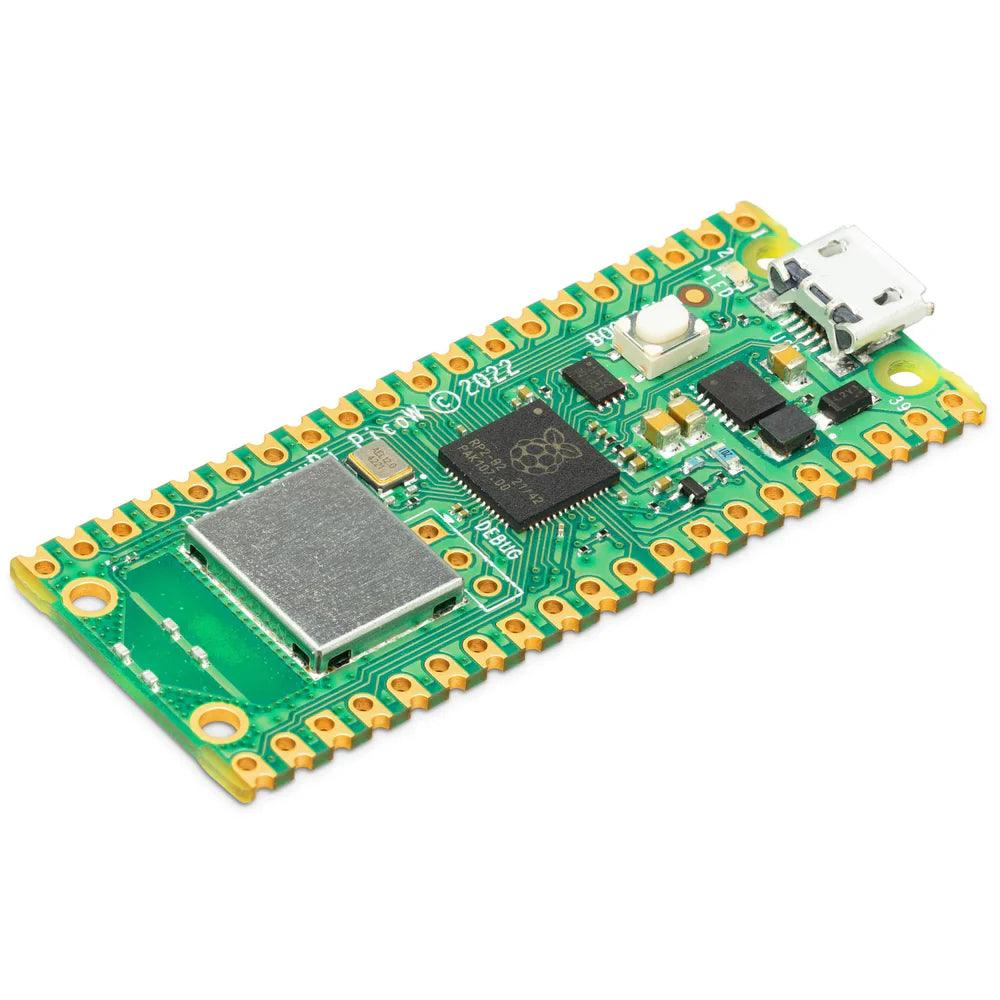
\includegraphics[width=\linewidth, keepaspectratio]{images/components/pico_w.jpg} & PCB: 2.1$\times$5.1 & RP2040, Dual-core ARM Cortex-M0+ @133MHz\newline \textbf{Voltage:} 1.8–5.5V, 3.3V logic\newline \textbf{Current:} ~91 mA (Wi-Fi active)\newline \textbf{Power:} Max ~0.5W \\ \hline

\href{https://www.ram-e-shop.com/shop/ro-motor-tt-mini-dc-gearbox-motors-pair-2-motors-with-back-shaft-9455}{\textbf{\textcolor{darkblue}{DC Motors (TT Mini Gearbox Pair)}}} & 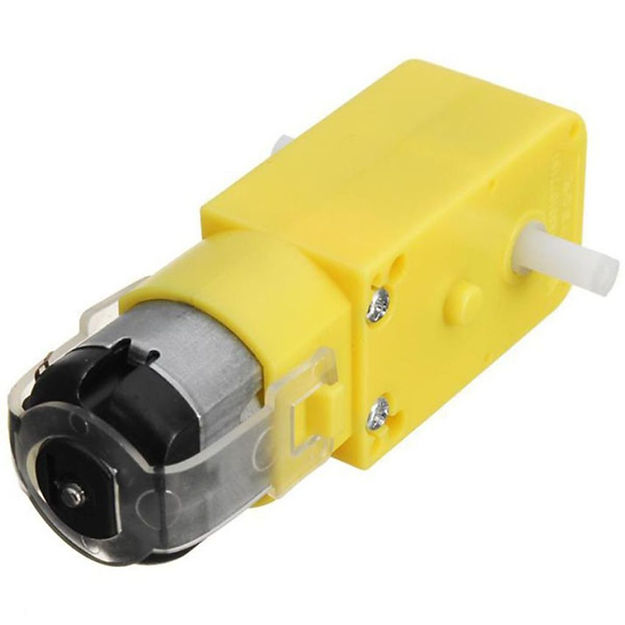
\includegraphics[width=\linewidth, keepaspectratio]{images/components/dc_motor_tt.jpg} & Per motor:\newline W2.2$ \newline \times$L7$\times$H1.8 & \textbf{No-load Speed:} 90 RPM\newline \textbf{Max Torque:} 800 gf.cm\newline \textbf{Voltage:} 3-12V\newline \textbf{No-load Current:} 190-250mA \\ \hline

\href{https://www.ram-e-shop.com/shop/kit-l298-red-l298-module-red-board-dual-h-bridge-motor-driver-using-l298n-7084}{\textbf{\textcolor{darkblue}{H-Bridge L298N Motor Driver}}}~\cite{L298NDatasheet, GeeetechL298NBoard} & 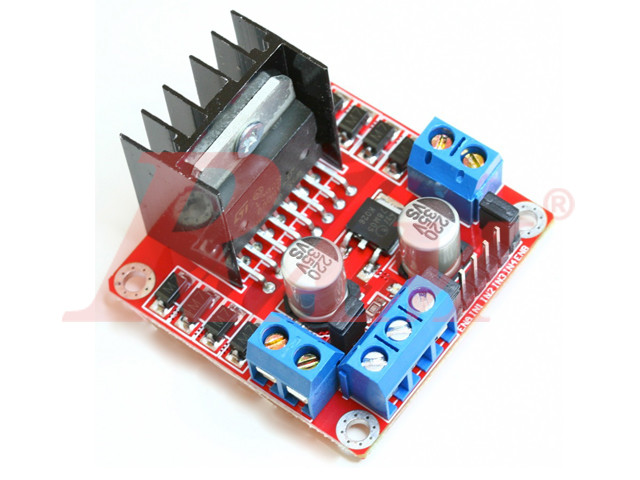
\includegraphics[width=\linewidth, keepaspectratio]{images/components/l298n_driver.jpg} & 4.3$\times$4.3$\times$2.7 & \textbf{Logic Voltage:} 5V\newline \textbf{Drive Voltage:} 5-35V\newline \textbf{Max Current:} 2A/channel\newline \textbf{Max Power:} 25W \\ \hline

\href{https://www.ram-e-shop.com/shop/kit-ultrasonic-hcsr04-ultrasonic-sensor-hc-sr04-5949}{\textbf{\textcolor{darkblue}{HC-SR04 Sensor}}}~\cite{HCSR04Datasheet} & 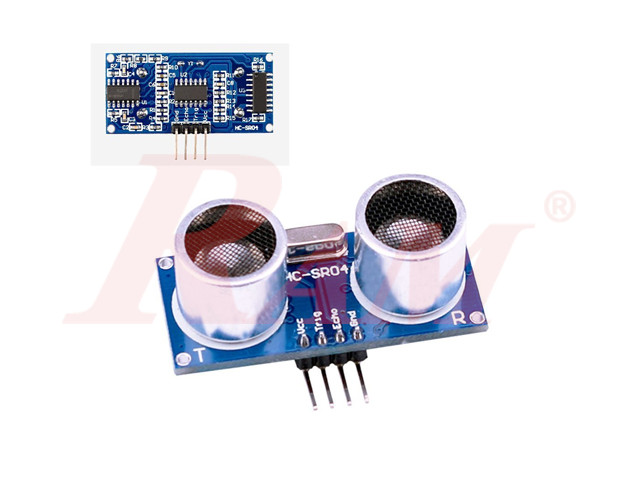
\includegraphics[width=\linewidth, keepaspectratio]{images/components/hcsr04_sensor.jpg} & W4.45 \newline $\times$H2$\times$D1.5 & \textbf{Voltage:} 5V DC\newline \textbf{Current:} $\sim$15mA\newline \textbf{Range:} 2cm - 400cm \\ \hline

\href{https://www.ram-e-shop.com/shop/battery-li-12v-4000mah-battery-pack-12v-4000mah-6728}{\textbf{\textcolor{darkblue}{Battery Pack}}}~\cite{BatteryPack12V4000mAhDatasheet} & 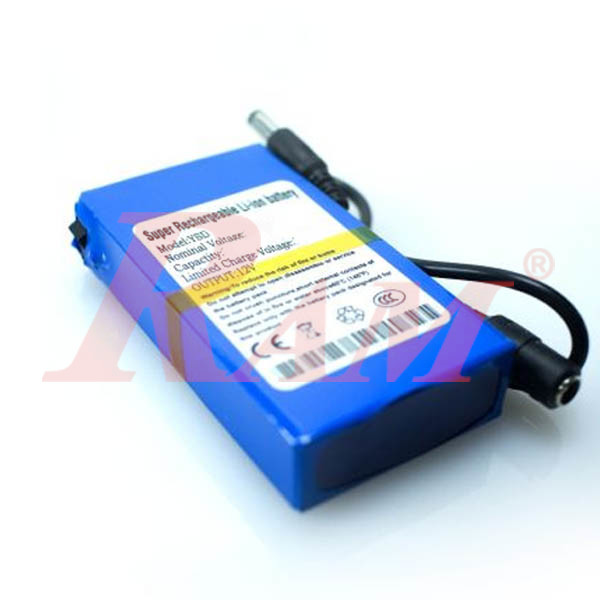
\includegraphics[width=\linewidth, keepaspectratio]{images/components/battery_12v.jpg} & 9.3$\times$6$\times$1.8 & \textbf{Output:} DC 2.1mm Jack\newline \textbf{Type:} \hyperref[term:liion]{Lithium-ion}\newline \textbf{Capacity:} 4000mAh @ 12V \\ \hline

\href{https://www.psdevwiki.com/ps3/Delta_KSB1012HE}{\textbf{\textcolor{darkblue}{PS3 Fan}}}~\cite{DeltaKSB1012HE_PSDevWiki} & 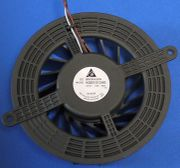
\includegraphics[width=\linewidth, keepaspectratio]{images/components/ps3_fan.jpg} & Diameter: $\sim$10 & \textbf{Voltage:} 12V DC\newline \textbf{Current:} $\sim$1.30A\newline \textbf{Connection:} 3-Pin (Pwr, Gnd, PWM Ctrl) \\ \hline

\href{https://www.ram-e-shop.com/shop/dc-dc-100-dc-dc-step-down-voltage-converter-adjustable-3a-lm2596s-4-38vdc-to-1-5-35vdc-sku-dc100-7257}{\textbf{\textcolor{darkblue}{DC-DC Step Down LM2596S}}}~\cite{LM2596SDatasheet} & 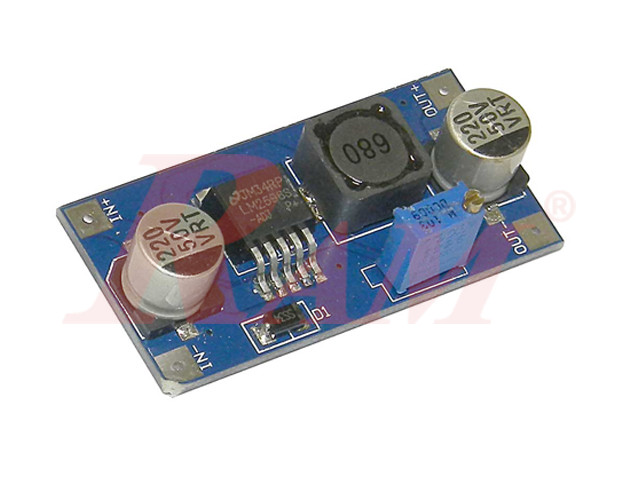
\includegraphics[width=\linewidth, keepaspectratio]{images/components/lm2596s_buck.jpg} & 4.35$\times$2.1$\times$1.4 & \textbf{Input:} 4-38V DC\newline \textbf{Output:} 1.5-35V DC (Adj.)\newline \textbf{Current:} 3A Max\newline \textbf{Frequency:} 150kHz \\ \hline

\href{https://homesensors.net/product/ir-photoelectric-encoder-sensor-4pin/}{\textbf{\textcolor{darkblue}{IR Photoelectric Encoder Sensor}}} & 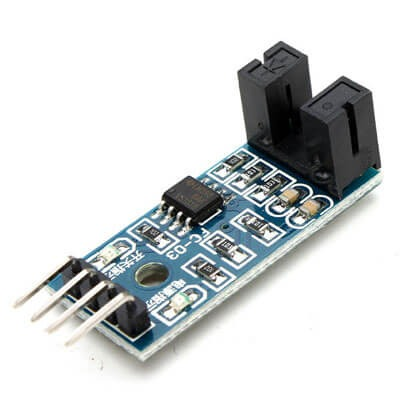
\includegraphics[width=\linewidth, keepaspectratio]{images/components/encoder_sensor.jpg} & 3.2$\times$1.4$\times$1.0 & \textbf{IC:} LM393\newline \textbf{Voltage:} 3.3-5.0V\newline \textbf{Groove Width:} 5mm\newline \textbf{Output:} Digital TTL \\ \hline

\href{https://homesensors.net/product/rotary-encoder-1pcs/}{\textbf{\textcolor{darkblue}{Rotary Encoder Disc}}} & 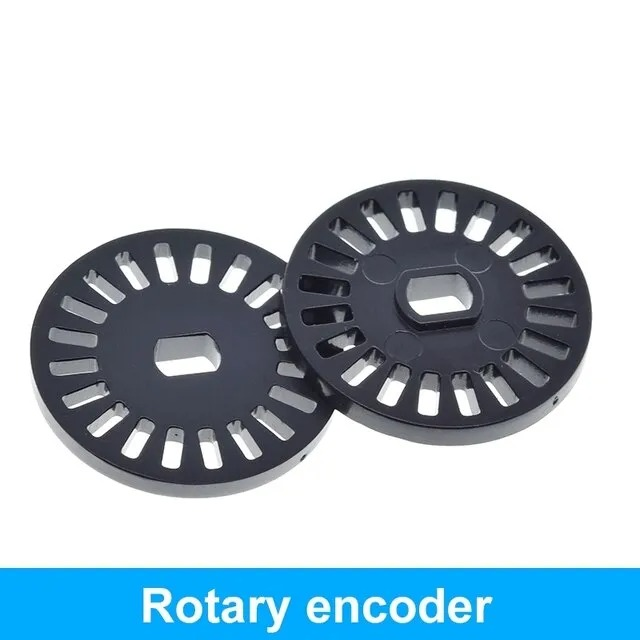
\includegraphics[width=\linewidth, keepaspectratio]{images/components/encoder_disc.jpg} & $\varnothing$: ~2.5 & \textbf{Material:} Plastic\newline \textbf{Slots:} 20 \\ \hline

\href{https://www.ram-e-shop.com/shop/pb-2-green-push-button-type-2-green-color-5614}{\textbf{\textcolor{darkblue}{Push Button (Green)}}} & 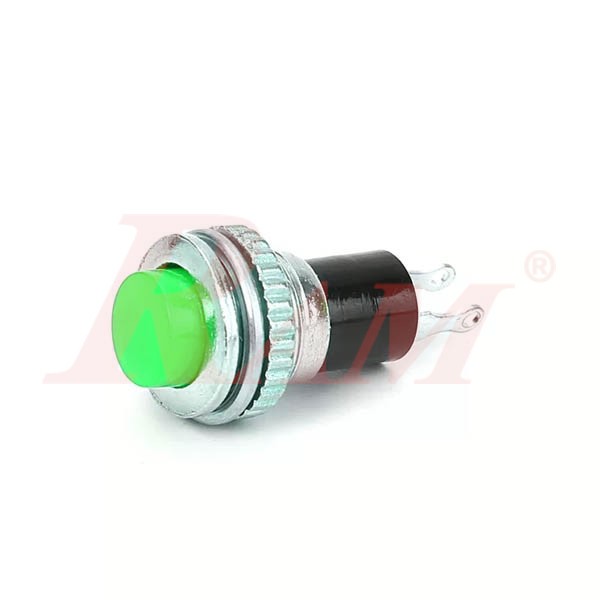
\includegraphics[width=\linewidth, keepaspectratio]{images/components/push_button_green.jpg} & Thread $\varnothing$: 9mm\newline Button $\varnothing$: 7mm\newline Overall: 1.2$\times$2.5 & \textbf{Type:} Momentary, Normally Open\newline \textbf{Rating:} AC 3A/125V, 1.5A/250V \\ \hline

\href{https://www.ram-e-shop.com/shop/xd10-3-12vdc-green-xd10-3-dc12v-green-small-led-signal-indicator-light-10mm-9155}{\textbf{\textcolor{darkblue}{LED Indicator}}} & 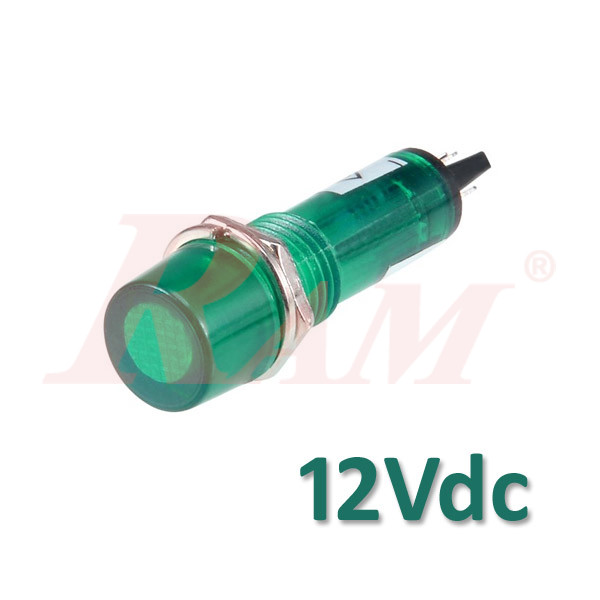
\includegraphics[width=\linewidth, keepaspectratio]{images/components/led_indicator.jpg} & Mount Hole $\varnothing$: 10mm\newline Overall: L4.15$\times\varnothing$1.15 & \textbf{Rated Voltage:} DC 12V\newline \textbf{Color:} Green \\ \hline

\href{https://www.ram-e-shop.com/shop/r-5-roseta-2pin-2-pin-pcb-screw-terminal-block-pitch-5mm-14-1mm-long-r-5-6323}{\textbf{\textcolor{darkblue}{2 Pin Screw Terminal}}} & 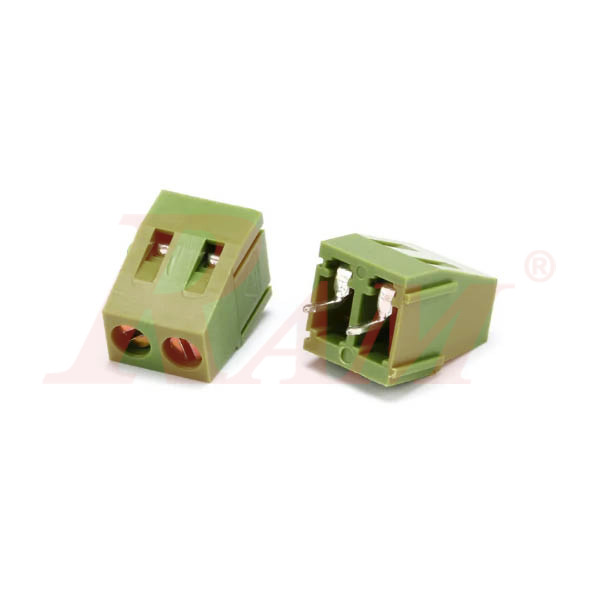
\includegraphics[width=\linewidth, keepaspectratio]{images/components/terminal_2pin.jpg} & Pitch: 0.5\newline Pin Dim: 0.43 & \textbf{Rating:} 24A / 250V\newline \textbf{Wire:} 26-14AWG \\ \hline

\href{https://www.ram-e-shop.com/shop/r-6-roseta-3pin-3-pin-pcb-screw-terminal-block-pitch-5mm-14-1mm-long-r-6-6322}{\textbf{\textcolor{darkblue}{3 Pin Screw Terminal}}} & 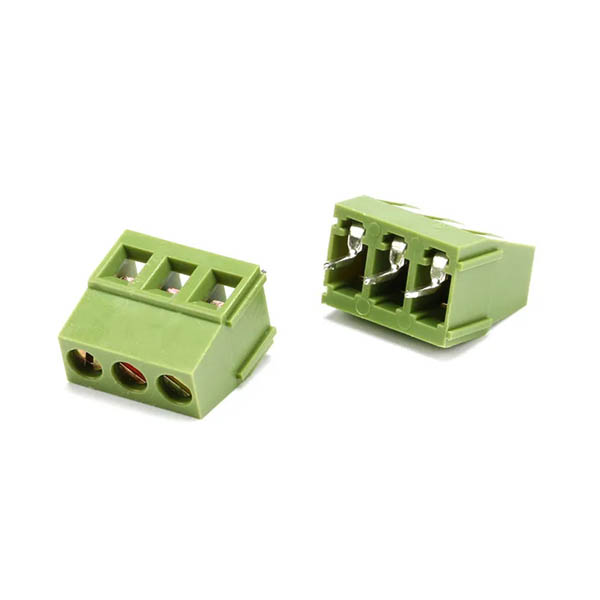
\includegraphics[width=\linewidth, keepaspectratio]{images/components/terminal_3pin.jpg} & Pitch: 0.5\newline Pin Dim: 0.43 & \textbf{Rating:} 24A / 250V\newline \textbf{Wire:} 26-14AWG \\ \hline

\href{https://www.ram-e-shop.com/shop/ph35-1x20-female-ph35-pin-header-female-1x20-straight-2-54mm-6529}{\textbf{\textcolor{darkblue}{Pin Header Female 1x20}}} & 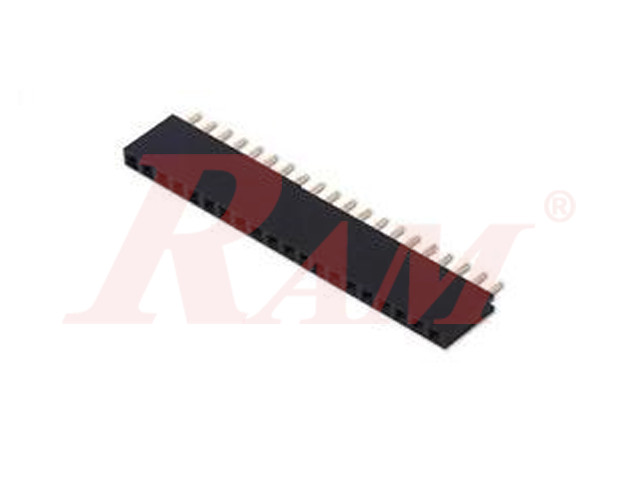
\includegraphics[width=\linewidth, keepaspectratio]{images/components/pin_header_female.jpg} & Spacing: 0.254 & \textbf{Configuration:} 1x20 Pins, Straight\newline \textbf{Current Rating:} 3A \\ \hline

\href{https://microohm-eg.com/product/6mm-electrical-waterproof-seal-heat-shrink-splice-wire-sleeve-yellow-1pcs/}{\textbf{\textcolor{darkblue}{Heat Shrink Sleeve (6mm Yellow)}}} & 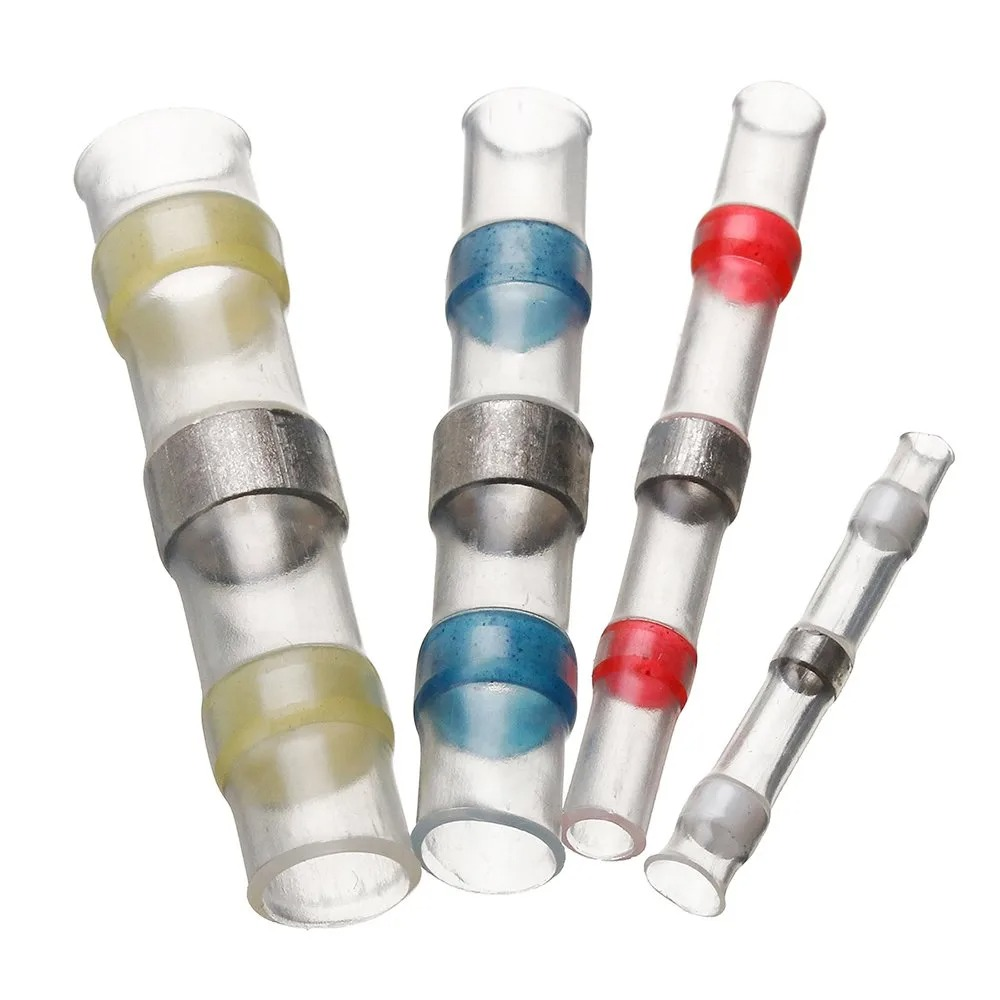
\includegraphics[width=\linewidth, keepaspectratio]{images/components/heat_shrink.jpg} & $\varnothing$: 0.6\newline Length: 4.0 & \textbf{Material:} Polyolefin\newline \textbf{Shrink Ratio:} 2:1, Waterproof \\ \hline

{\textbf{\textcolor{darkblue}{Resistor 2.2k$\Omega$}}} & 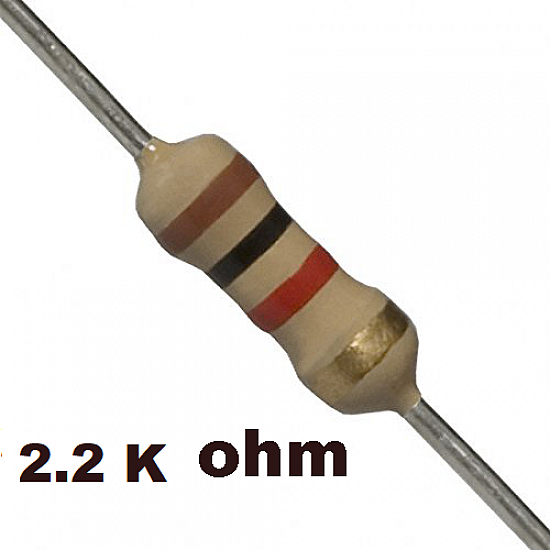
\includegraphics[width=\linewidth, keepaspectratio]{images/components/resistor_2k2.png} & Axial Pkg. & \textbf{Value:} 2.2k$\Omega$\newline \textbf{Power:} 1/4W\newline \textbf{Type:} Axial \\ \hline

{\textbf{\textcolor{darkblue}{Resistor 4.7k$\Omega$}}} & 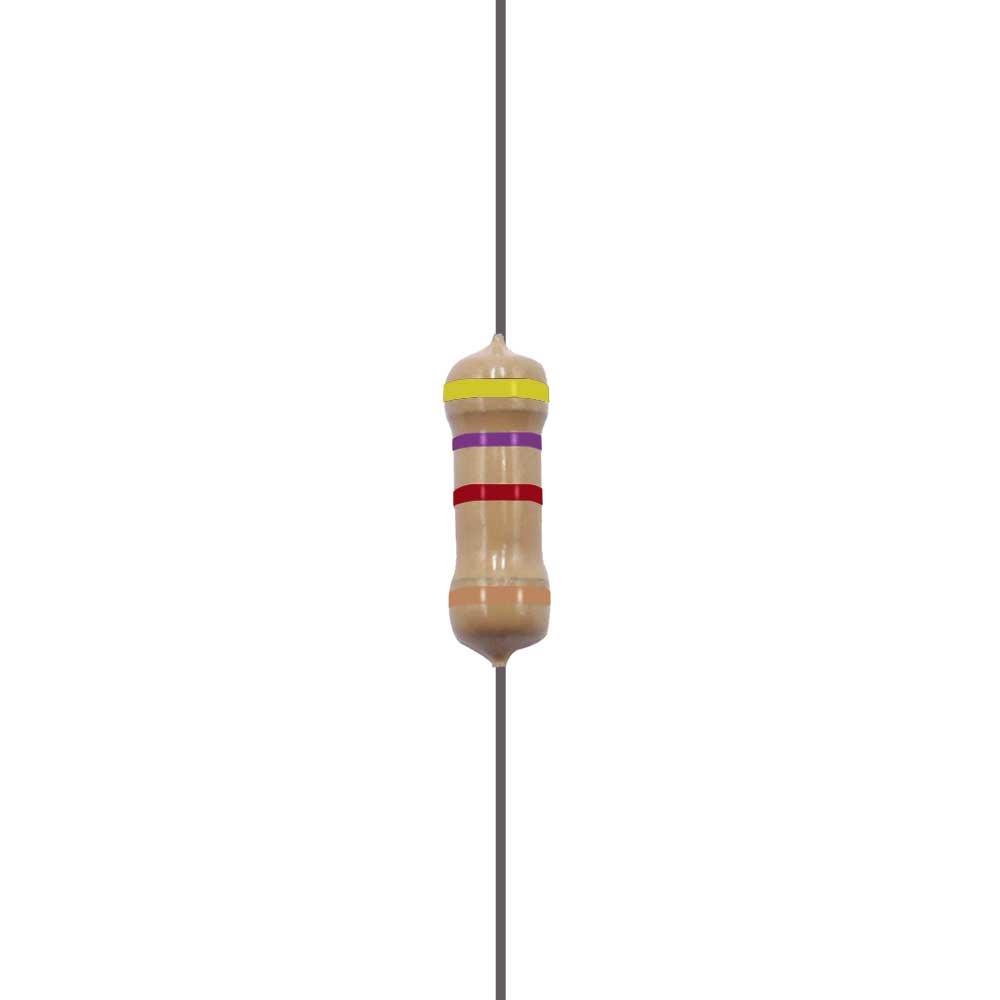
\includegraphics[width=\linewidth, keepaspectratio]{images/components/resistor_4k7.jpg} & Axial Pkg. & \textbf{Value:} 4.7k$\Omega$\newline \textbf{Power:} 1/4W\newline \textbf{Type:} Axial \\ \hline

\href{https://www.ram-e-shop.com/shop/ph60-mf-20cm-ph60-20cm-male-to-female-40-jumper-wires-set-7066}{\textbf{\textcolor{darkblue}{Jumper Wires M-F}}} & 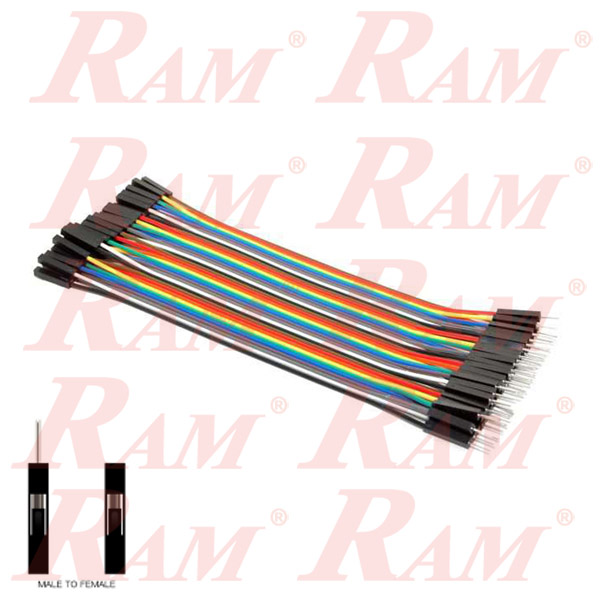
\includegraphics[width=\linewidth, keepaspectratio]{images/components/jumper_mf.jpg} & Length: 20 & \textbf{Configuration:} Male-to-Female\newline \textbf{Quantity:} 40 Wires\newline \textbf{Current Rating:} 1A \\ \hline

\href{https://www.ram-e-shop.com/shop/ph61-mm-20cm-ph61-20cm-male-to-male-40-jumper-wires-set-7094}{\textbf{\textcolor{darkblue}{Jumper Wires M-M}}} & 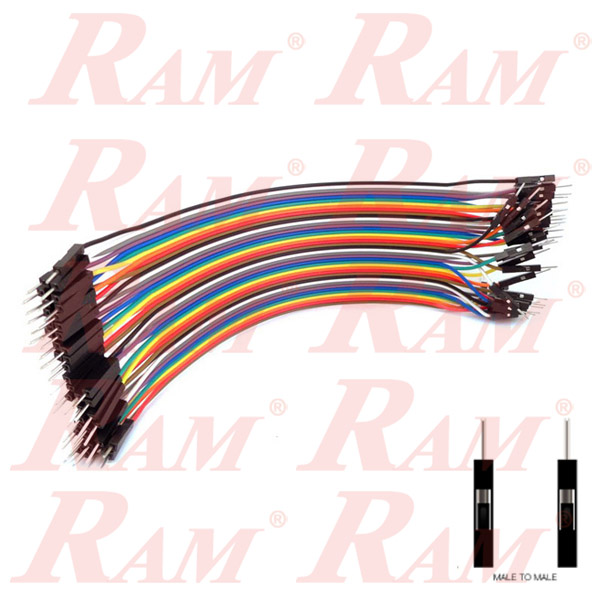
\includegraphics[width=\linewidth, keepaspectratio]{images/components/jumper_mm.jpg} & Length: 20 & \textbf{Configuration:} Male-to-Male\newline \textbf{Quantity:} 40 Wires\newline \textbf{Current Rating:} 1A \\ \hline

\href{https://www.ram-e-shop.com/shop/ph62-ff-20cm-ph62-20cm-female-to-female-40-jumper-wires-set-7189}{\textbf{\textcolor{darkblue}{Jumper Wires F-F}}} & 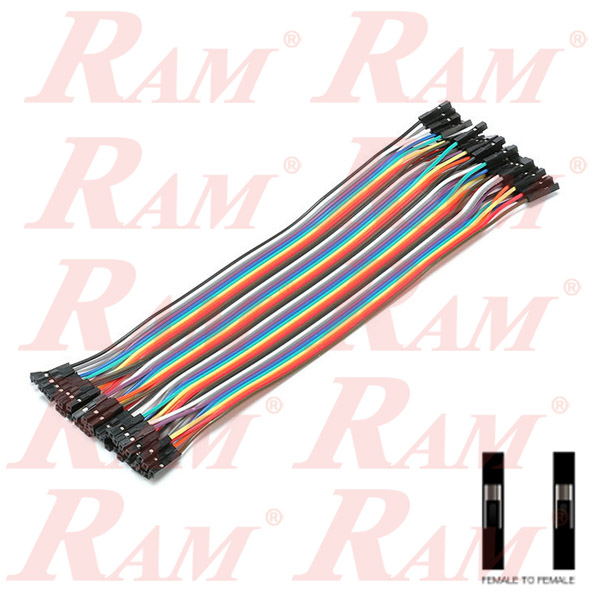
\includegraphics[width=\linewidth, keepaspectratio]{images/components/jumper_ff.jpg} & Length: 20 & \textbf{Configuration:} Female-to-Female\newline \textbf{Quantity:} 40 Wires\newline \textbf{Current Rating:} 1A \\ \hline

\href{https://www.ram-e-shop.com/shop/wire-speaker-2x1mm-speaker-wire-2-core-x-1mm-red-black-1-meter-8878}{\textbf{\textcolor{darkblue}{Speaker Wire}}} & 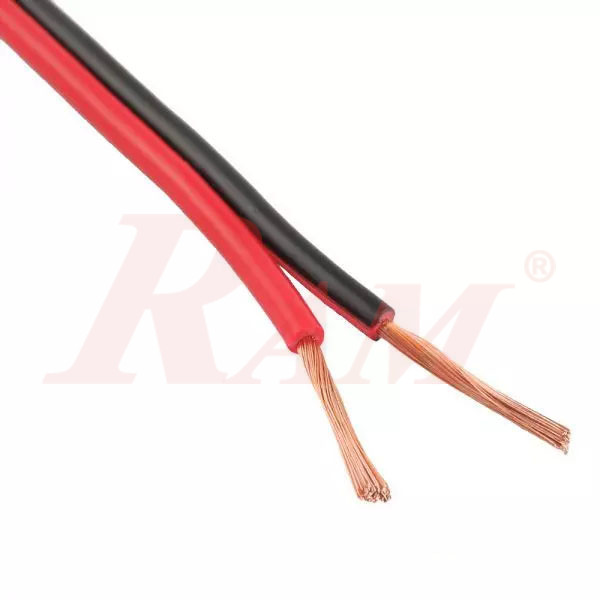
\includegraphics[width=\linewidth, keepaspectratio]{images/components/speaker_wire.jpg} & Size: 2Cx0.1\newline Length: 100 (per meter) & \textbf{Colors:} Red \& Black\newline \textbf{Material:} OFC Copper, PVC Jacket \\ \hline

\end{longtable}
\fussy % Return to normal spacing behavior after the table
\endgroup

\section{System Architecture}
\label{sec:system_architecture_ctrl_new} % Relabelled from old sec:system_architecture_ctrl
The robot's control system is centralized around the Raspberry Pi Pico W microcontroller~\cite{PicoWDatasheet}. This board was chosen for its dual-core ARM Cortex-M0+ processor, sufficient \hyperref[term:gpio]{GPIO} pins, integrated Wi-Fi and \hyperref[term:ble]{BLE} capabilities (Pico W variant), low cost, and robust MicroPython support~\cite{RpiPicoSeriesDocs}. A pinout diagram for the Raspberry Pi Pico W is shown in Figure~\ref{fig:pico_w_pinout_diagram_new}. The Pico W is responsible for:
\begin{itemize}
    \item Reading and processing data from the \hyperref[term:hcsr04]{HC-SR04} ultrasonic sensor for obstacle detection.
    \item Processing high-frequency interrupt signals from two wheel encoders for odometry.
    \item Controlling the two \hyperref[term:dc]{DC} gear motors via an \hyperref[term:l298n]{L298N} H-bridge motor driver, using a \hyperref[term:pid]{PID} algorithm for precise motion control.
    \item Managing the operation of the 12V PS3 fan.
    \item Handling user input from a physical start/stop button.
    \item Providing status feedback via an \hyperref[term:led]{LED} indicator.
    \item Managing \hyperref[term:ble]{BLE} communication for remote control via a smartphone application like NRF Toolbox.
\end{itemize}

Figure~\ref{fig:system_block_diagram} provides a high-level overview of the autonomous cleaning control flow, illustrating how the system transitions between user commands, forward motion with hybrid feed-forward and PID control, obstacle detection, and stall recovery.

\begin{figure}[htbp]
\centering
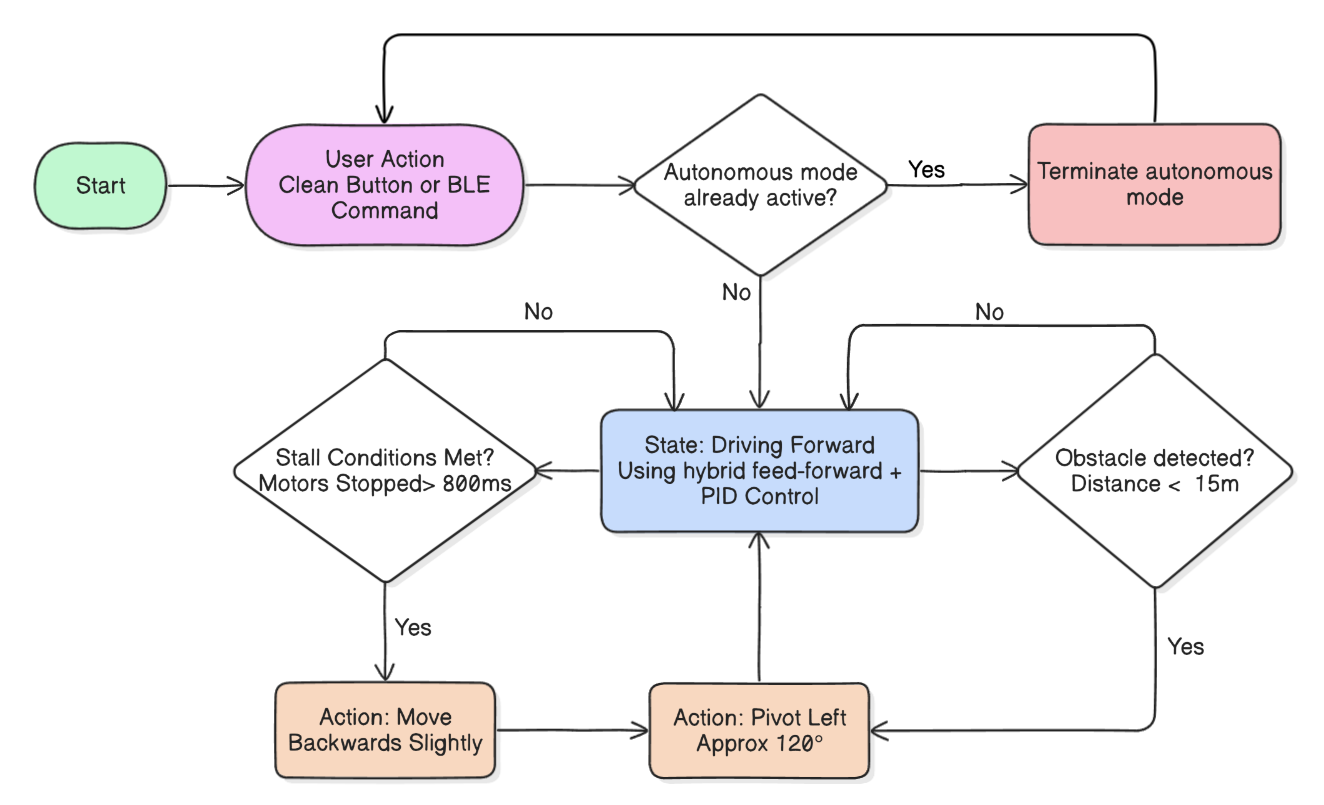
\includegraphics[width=\textwidth]{images/screenshots/control_flowchart.png}
\caption{High-level control flowchart of the autonomous cleaning mode, showing user-initiated activation, forward motion with hybrid PID control, obstacle avoidance, and stall recovery paths.}
\label{fig:system_block_diagram}
\end{figure}

\begin{sidewaysfigure}
    \centering
    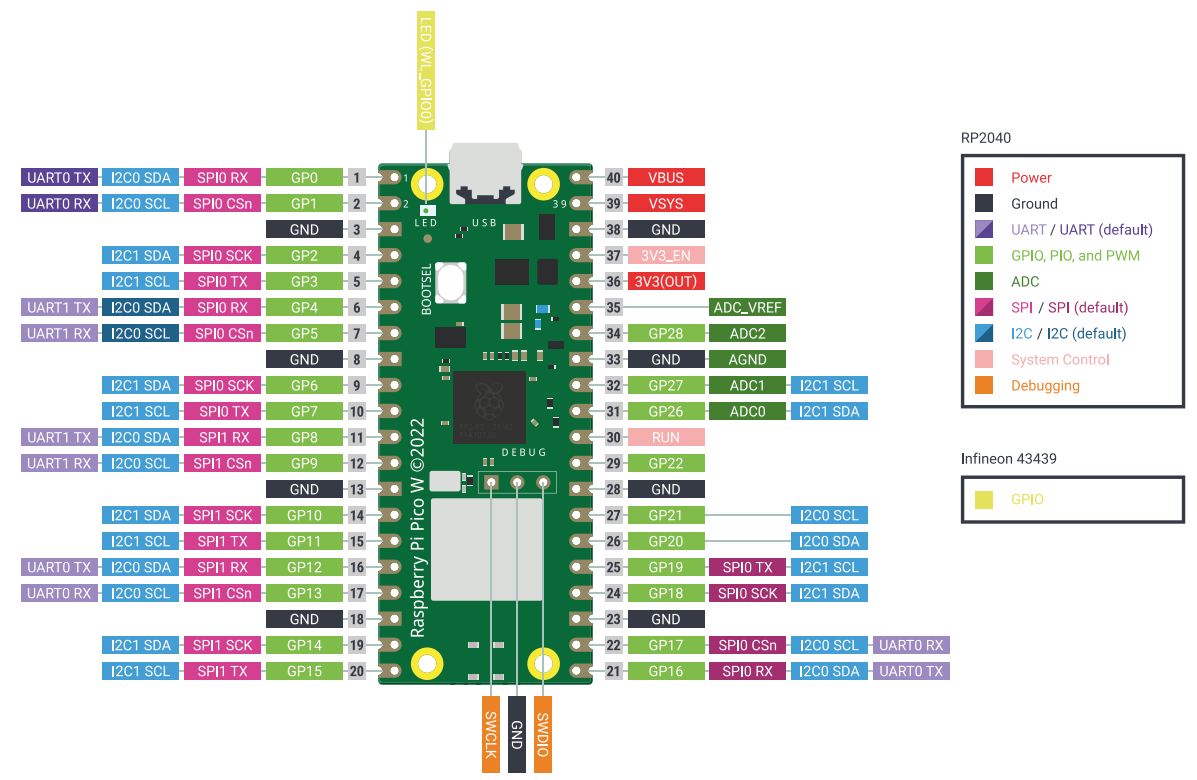
\includegraphics[width=1\textwidth, keepaspectratio]{images/screenshots/pico_w_pinout.png}
    \caption{Raspberry Pi Pico W pinout diagram. Source:~\cite{PicoWDatasheet}.}
    \label{fig:pico_w_pinout_diagram_new} % Relabelled from fig:pico_w_pinout_diagram
\end{sidewaysfigure}


\section{Electrical Design and Integration}
\label{sec:electrical_design_integration_new}
The electrical design focuses on safely and reliably interconnecting all electronic components, culminating in a custom \hyperref[term:pcb]{PCB} for a robust final assembly.
\subsection{Power Distribution}
\label{subsec:power_distribution_new}
\begin{itemize}
    \item The 12V \hyperref[term:liion]{Li-ion} battery~\cite{BatteryPack12V4000mAhDatasheet} is the primary power source.
    \item The LM2596S buck converter~\cite{LM2596SDatasheet} steps down the 12V to a regulated 5V. This 5V rail powers:
        \begin{itemize}
            \item The Raspberry Pi Pico W via its VSYS pin.
            \item The logic side of the \hyperref[term:l298n]{L298N} motor driver (Vss or +5V pin).
            \item The \hyperref[term:hcsr04]{HC-SR04} ultrasonic sensor (VCC pin).
            \item The two IR photoelectric encoder sensors (VCC pins).
        \end{itemize}
    \item The 12V from the battery directly powers:
        \begin{itemize}
            \item The motor input (Vs or VM) of the \hyperref[term:l298n]{L298N} module.
            \item The PS3 fan.
        \end{itemize}
    \item A common ground (GND) is maintained across all components.
\end{itemize}

\subsection{Component Interconnections and Wiring}
\label{subsec:component_interconnections_wiring_new}
The Raspberry Pi Pico W’s \hyperref[term:gpio]{GPIO} pins are used for all control signals and sensor inputs. Key connections are detailed in the accompanying MicroPython source code (\texttt{main.py}) and visualized in the schematic diagrams (see Section~\ref{subsec:custom_pcb_design_new}). The specific \hyperref[term:gpio]{GPIO} assignments are as follows:

\begin{itemize}
    \item \textbf{Motor Control (\hyperref[term:l298n]{L298N})}: Six \hyperref[term:gpio]{GPIO} pins from the Pico W control the \hyperref[term:l298n]{L298N} driver~\cite{L298NDatasheet}:
        \begin{itemize}
            \item Left Motor PWM (ENA): GP6
            \item Left Motor Direction 1 (IN1): GP12
            \item Left Motor Direction 2 (IN2): GP13
            \item Right Motor PWM (ENB): GP7
            \item Right Motor Direction 1 (IN3): GP14
            \item Right Motor Direction 2 (IN4): GP15
        \end{itemize}

    
    \item \textbf{Wheel Encoder Inputs}: To facilitate the closed-loop control system, the wheel encoders were connected directly to interrupt-capable GPIO pins:
        \begin{itemize}
            \item Left Encoder Sensor: GP21
            \item Right Encoder Sensor: GP20
        \end{itemize}
        These pins were configured with internal pull-ups in the software to ensure a stable signal.
    \item \textbf{Ultrasonic Sensor (\hyperref[term:hcsr04]{HC-SR04})}:
        \begin{itemize}
            \item TRIG (Output): GP10
            \item ECHO (Input): GP11
        \end{itemize}
        A voltage divider circuit (e.g., 2.2k$\Omega$ and 4.7k$\Omega$ resistors) is used on the ECHO pin to safely step down the sensor’s 5V output to the Pico W’s 3.3V logic level.
    \item \textbf{PS3 Fan}: The fan’s \hyperref[term:pwm]{PWM} control pin (Grey wire) is connected to GP8 on the Pico W. While this hardware connection could support future software-based \hyperref[term:pwm]{PWM} speed control, the current prototype implements simple on/off control using this pin (leaving software-based speed control as a potential future enhancement). The fan’s +12V (Brown) and GND (Black) wires are connected to the 12V power supply.
    \item \textbf{User Interface}:
        \begin{itemize}
            \item Push Button (Start/Stop): GP16 (configured with an internal pull-up resistor).
            \item \hyperref[term:led]{LED} Indicator: GP18 (connected via a suitable current-limiting resistor as required).
        \end{itemize}
\end{itemize}


Initial conceptual validation of the control logic, particularly for obstacle avoidance, was performed using Proteus simulation (Figure~\ref{fig:combined_sim_breadboard}(a)). An Arduino Uno model was employed in the simulation due to the unavailability of a Raspberry Pi Pico W model in Proteus at the time of testing; this allowed for early verification of the fundamental sensor-driven decision-making processes. Following this simulation-based logic testing, the actual electrical connections for the chosen components were physically validated on a breadboard (Figure~\ref{fig:combined_sim_breadboard}(b)) before committing to the \hyperref[term:pcb]{PCB} design.
\begin{figure}[htbp]
    \centering
    \begin{subfigure}[b]{0.496\textwidth}
        \centering
        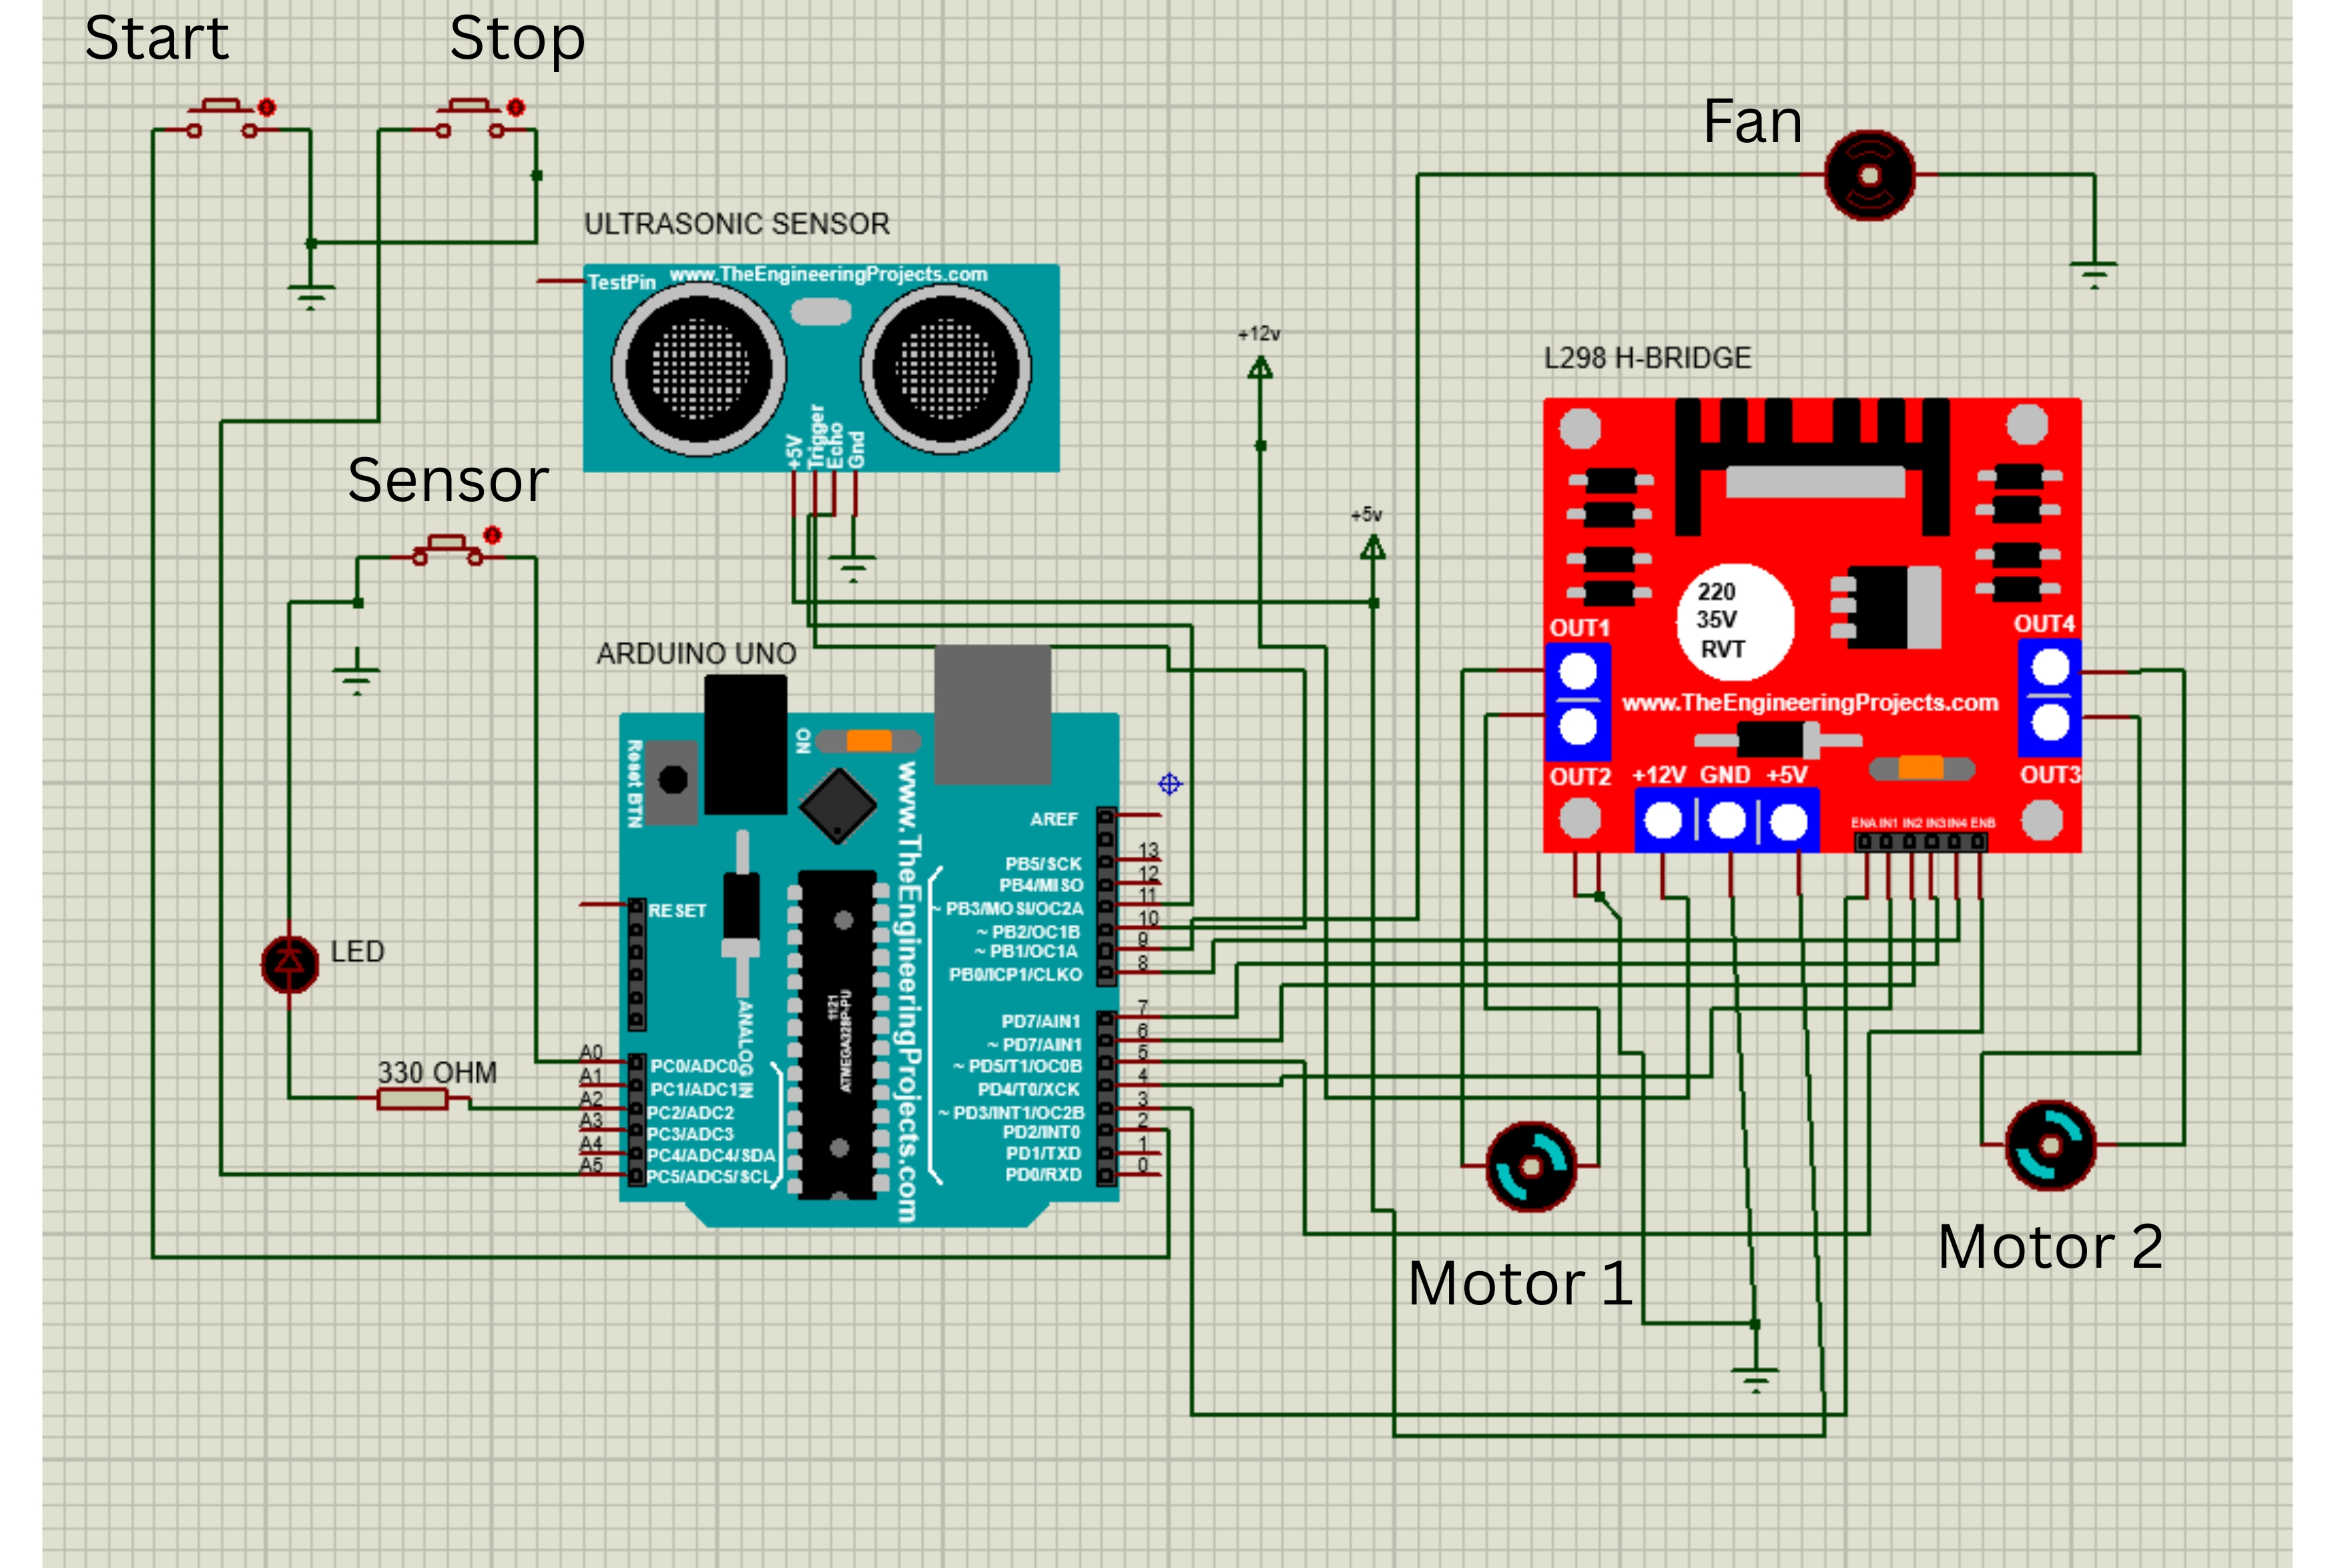
\includegraphics[width=\linewidth, keepaspectratio]{images/photos/proteus_simulation_shot.jpg}
        \caption{Proteus simulation of basic obstacle avoidance logic.}
        \label{fig:proteus_simulation_sub}
    \end{subfigure}
    \hfill % For spacing between subfigures
    \begin{subfigure}[b]{0.496\textwidth}
        \centering
        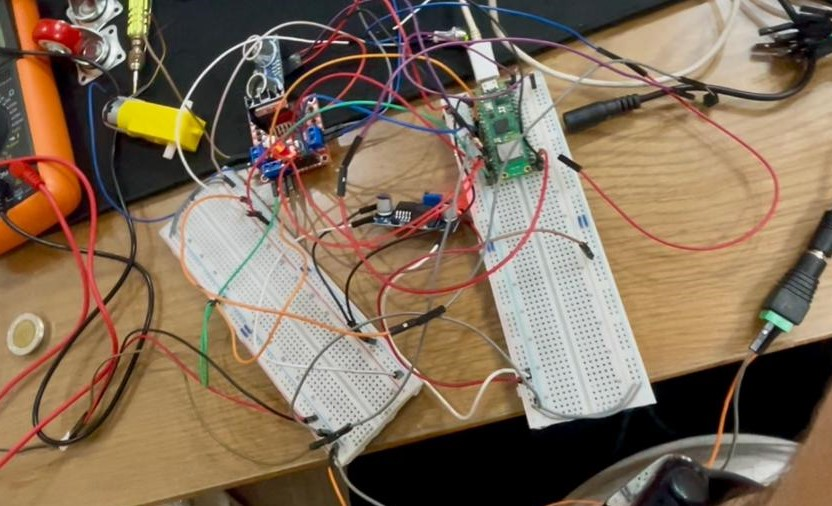
\includegraphics[width=\linewidth, keepaspectratio]{images/photos/breadboard_proto_shot.jpg}
        \caption{Breadboard prototype for physical validation.}
        \label{fig:breadboard_prototype_sub}
    \end{subfigure}
    \caption{Conceptual validation stages: (a) Proteus simulation of the robot's basic obstacle avoidance logic using an Arduino model, and (b) photograph of the breadboard prototype showing key component interconnections for physical validation.}
    \label{fig:combined_sim_breadboard}
\end{figure}

With the mechanical structure assembled, final electrical connections were made. Appropriate gauge wires were used for signal and power lines. Connections were double-checked for polarity and correctness against the wiring diagrams. Wire management involved routing cables to prevent interference with moving parts. Figure~\ref{fig:internal_wiring_photo_eval_new} shows the internal wiring with the custom \hyperref[term:pcb]{PCB}.
\begin{figure}[htbp]
    \centering
    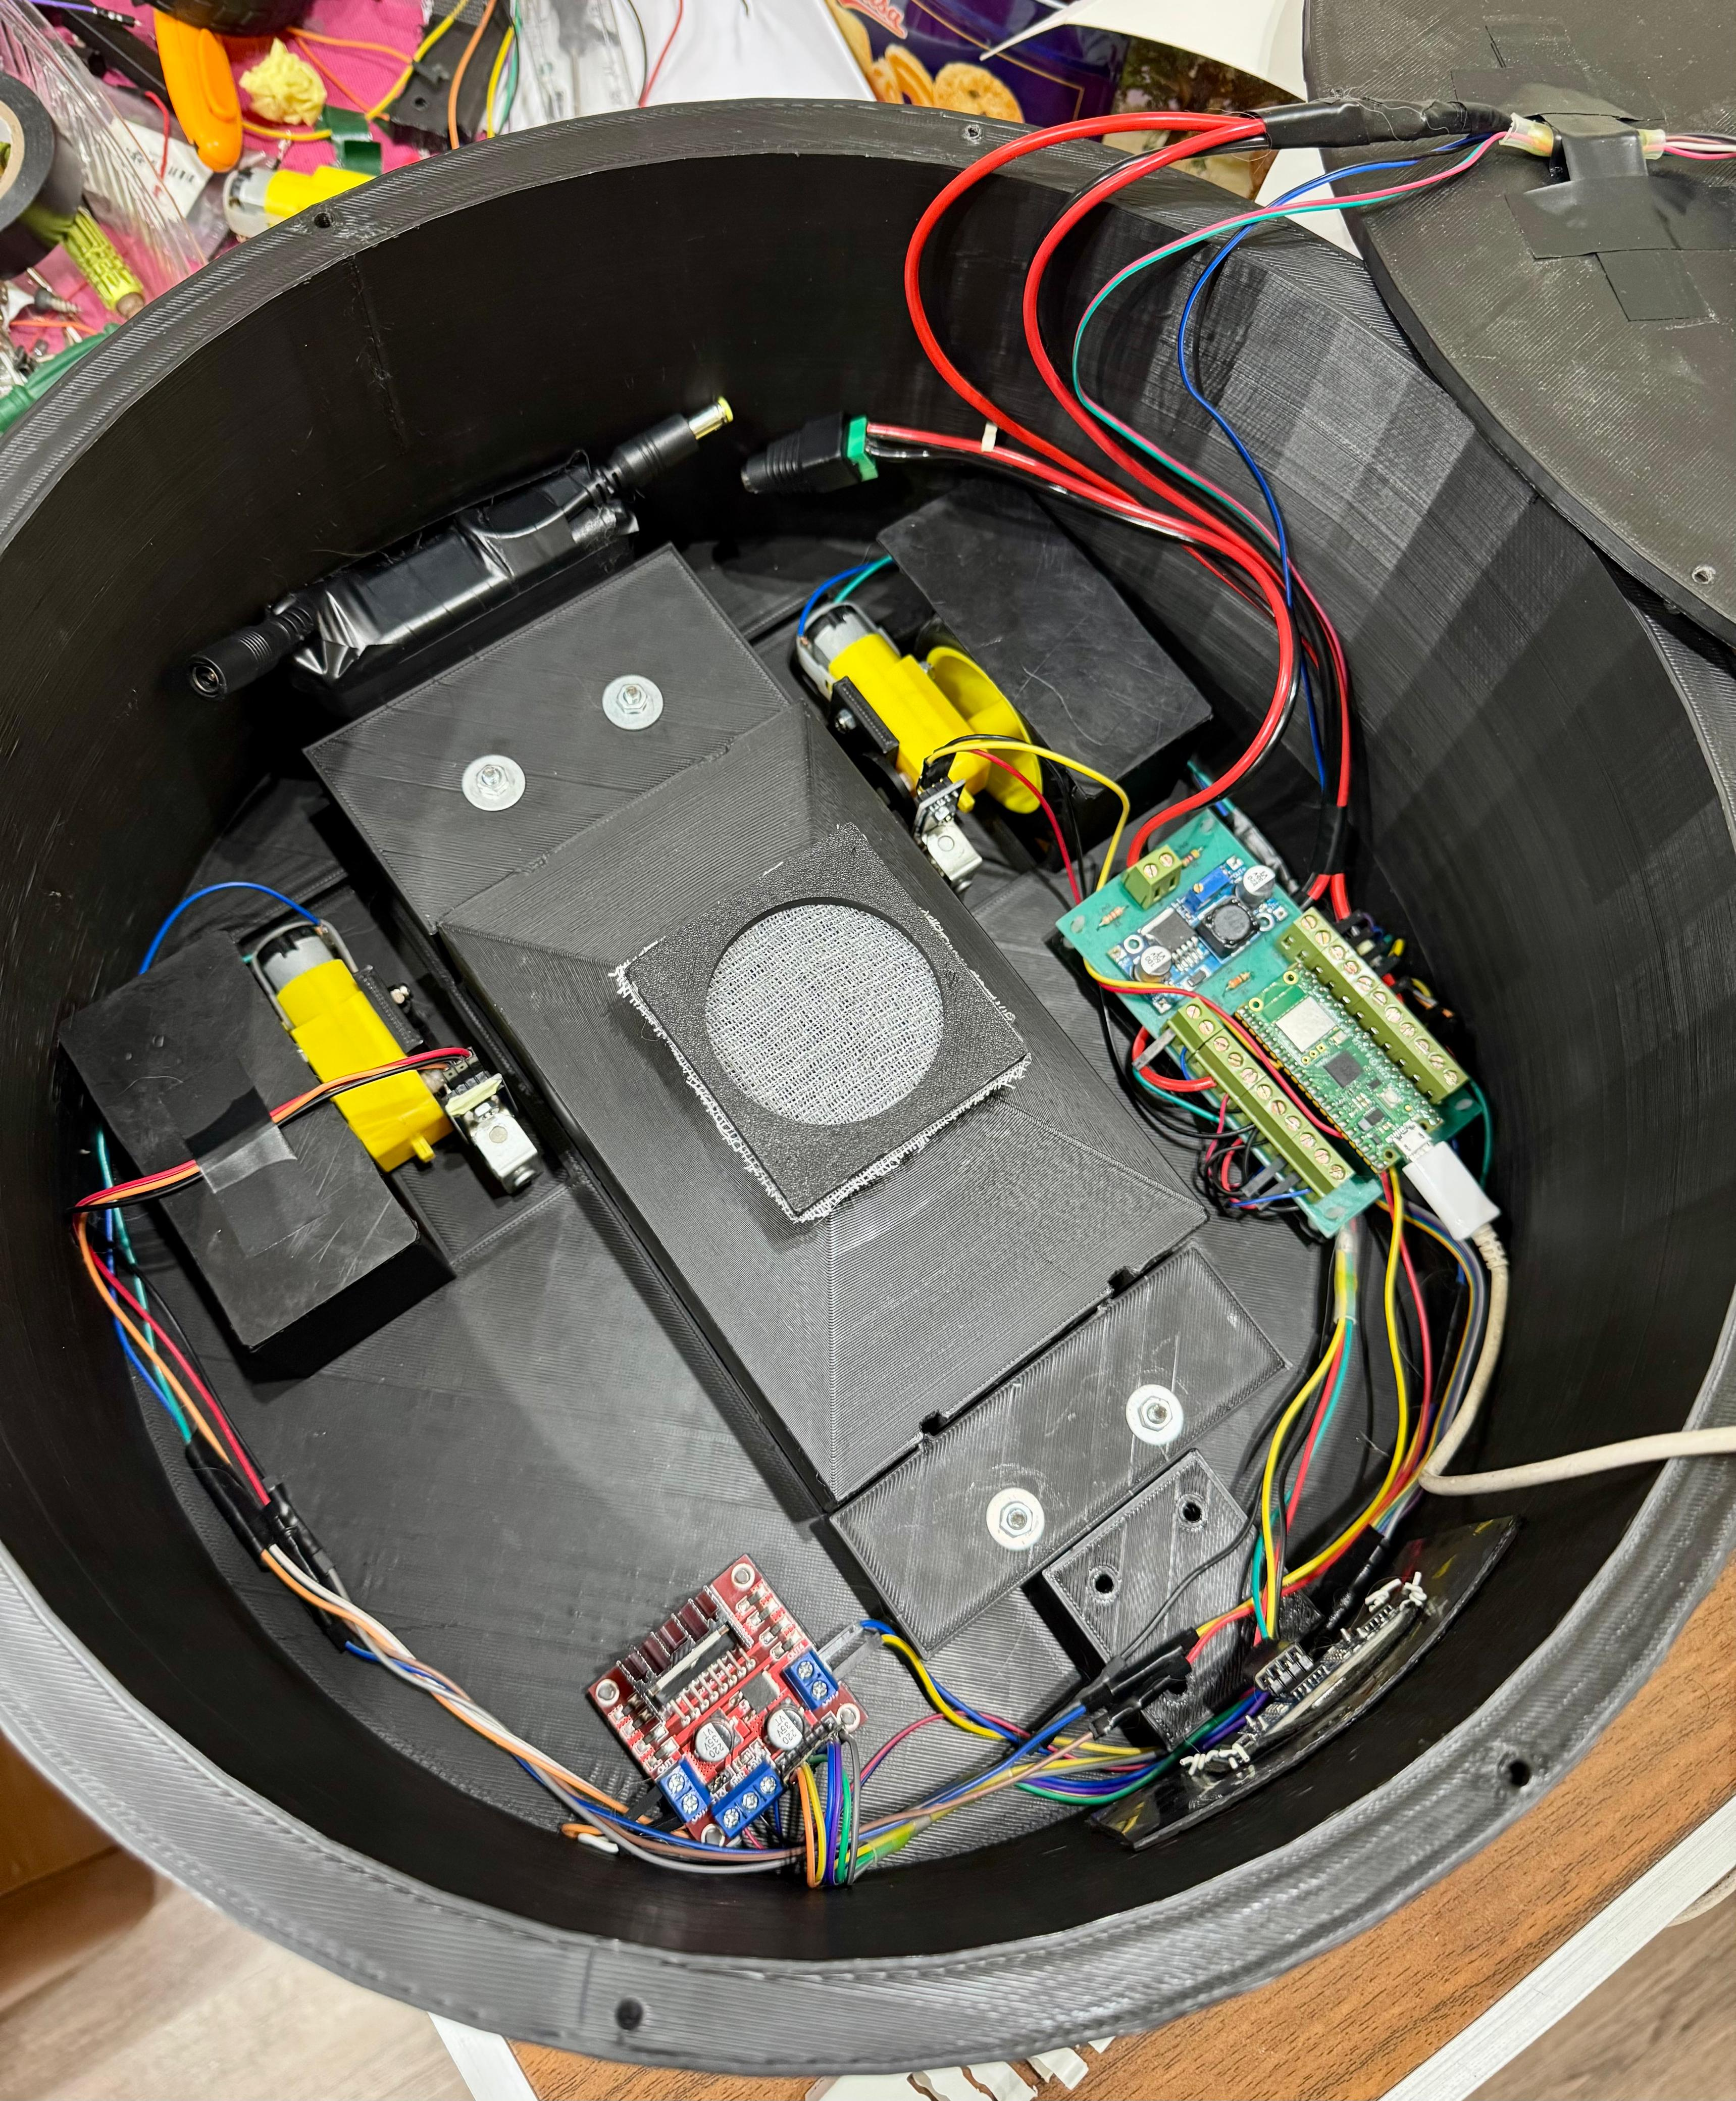
\includegraphics[width=\textwidth, keepaspectratio]{images/photos/internal_wiring.jpg}
    \caption{Internal view of the assembled robot showing component wiring and integration with the custom PCB.}
    \label{fig:internal_wiring_photo_eval_new} % Relabelled from fig:internal_wiring_photo_eval
\end{figure}


\subsection{Custom PCB Design and Fabrication}
\label{subsec:custom_pcb_design_new}
A custom 2-layer \hyperref[term:pcb]{PCB} (100mm x 50mm, FR4, 1oz copper, green solder mask, black legend) was designed in KiCad to integrate the Raspberry Pi Pico W, the LM2596S buck converter, screw terminals for external connections (motors, fan, sensor, button, \hyperref[term:led]{LED}), and the \hyperref[term:hcsr04]{HC-SR04} voltage divider circuit. This provided a more robust and organized solution than breadboard or perfboard wiring for the final prototype. The custom \hyperref[term:pcb]{PCB} served as the central point for connections, utilizing screw terminals for robust wiring to off-board components. The schematic, layout, and a 3D render of the \hyperref[term:pcb]{PCB} are shown in Figures \ref{fig:kicad_schematic_ctrl_new}, \ref{fig:kicad_layout_ctrl_new}, and \ref{fig:kicad_3d_render_ctrl_new} respectively.

It is important to note that the wheel encoders were integrated into the design as a post-manufacturing upgrade to enhance the robot's capabilities. Consequently, their wiring was connected directly to the Raspberry Pi Pico W's GPIO pins and is not reflected in the PCB schematic or layout diagrams (Figures \ref{fig:kicad_schematic_ctrl_new}, \ref{fig:kicad_layout_ctrl_new}).
\begin{figure}[htbp]
    \centering
    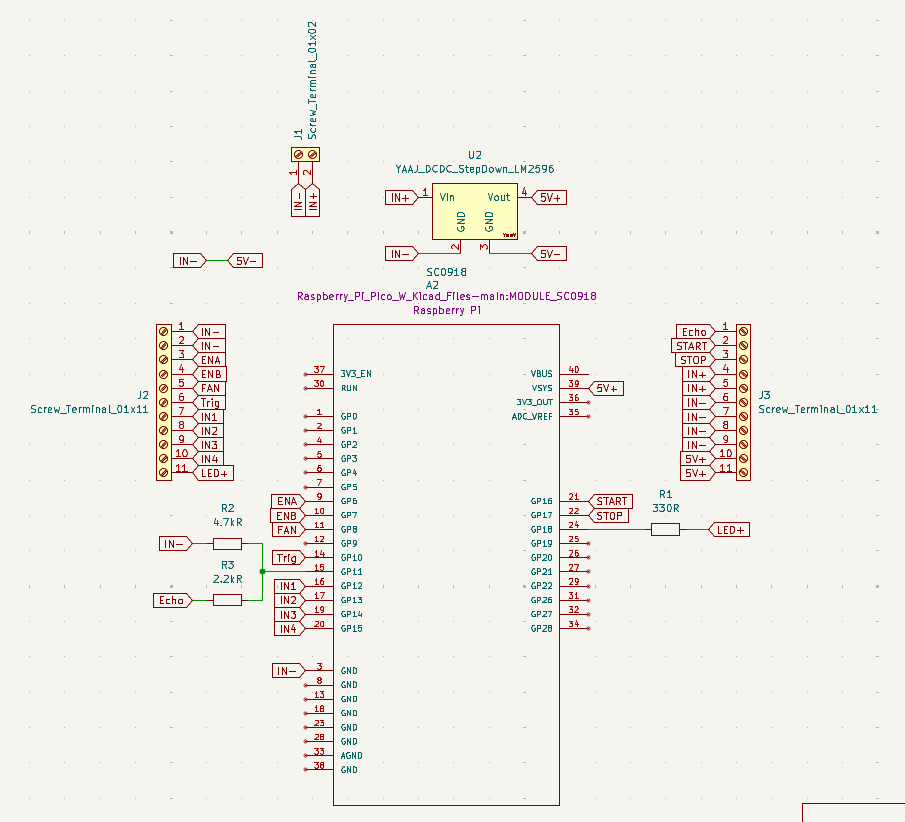
\includegraphics[width=\textwidth, keepaspectratio]{images/screenshots/kicad_schematic.png}
    \caption{KiCad schematic diagram for the custom Printed Circuit Board.}
    \label{fig:kicad_schematic_ctrl_new} % Relabelled from fig:kicad_schematic_ctrl
\end{figure}

\begin{figure}[htbp]
    \centering
    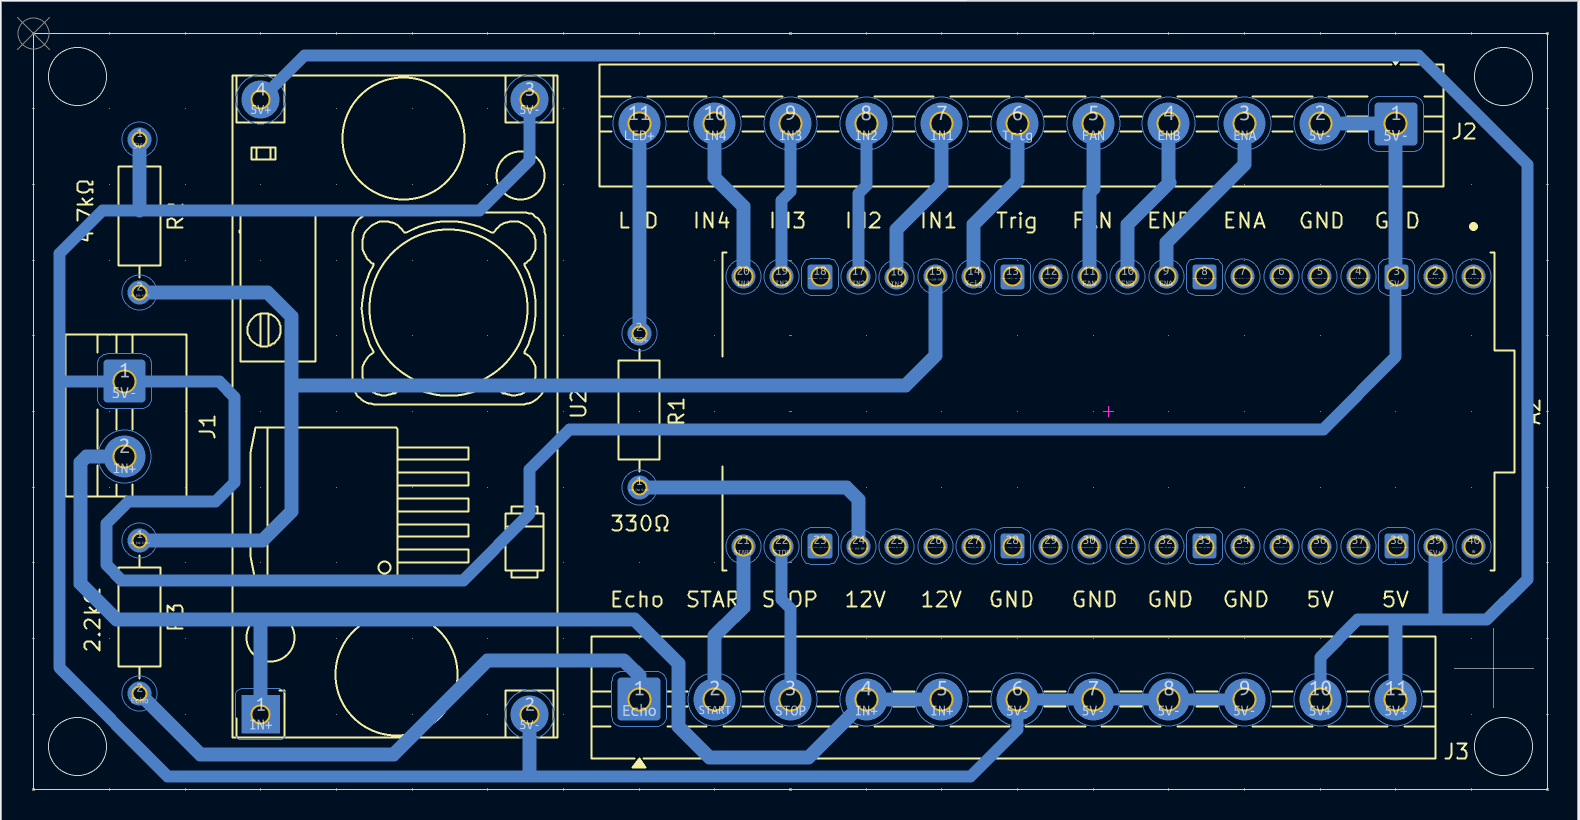
\includegraphics[width=0.928\textwidth, keepaspectratio]{images/screenshots/kicad_layout.png}
    \caption{KiCad PCB layout design (2D view).}
    \label{fig:kicad_layout_ctrl_new} % Relabelled from fig:kicad_layout_ctrl
\end{figure}

\begin{figure}[htbp]
    \centering
    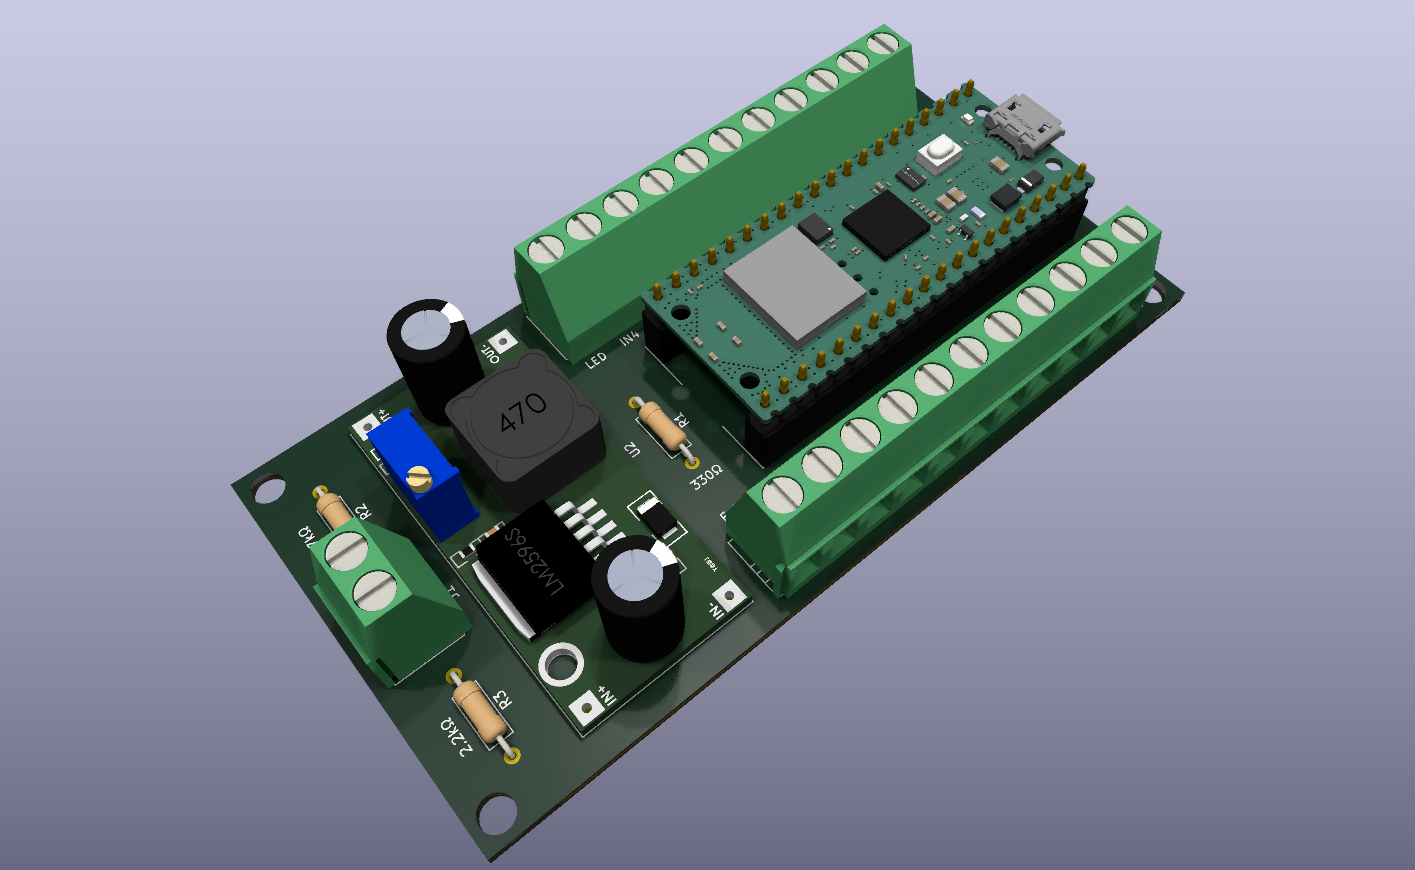
\includegraphics[width=0.928\textwidth, keepaspectratio]{images/screenshots/kicad_3d_render.png}
    \caption{3D rendering of the populated PCB design from KiCad.}
    \label{fig:kicad_3d_render_ctrl_new} % Relabelled from fig:kicad_3d_render_ctrl
\end{figure}

\section{Control System Implementation (Software)}
\label{sec:control_implementation_software_ctrl_new} % Relabelled from old sec:control_implementation_software_ctrl
The robot's behavior is governed by software developed in MicroPython, running on the Raspberry Pi Pico W. The complete source code is provided as an accompanying file (\texttt{code\_backup/main.py}).
\subsection{Software Architecture}
\label{subsec:software_architecture_new}
The software is structured modularly to handle various tasks:
\begin{itemize}
    \item \textbf{Hardware Abstraction Layer}: Functions to initialize and interact with hardware peripherals, including hardware interrupt handlers for the wheel encoders.
    \item \textbf{\hyperref[term:pid]{PID} Control Module}: Contains the feed-forward PWM calculation (\texttt{ff\_pwm}), straight-line motion with positional PID (\texttt{straight\_motion}), and pivot turns with a dual progress/balance PID (\texttt{pivot\_motion}).
    \item \textbf{Autonomous State Machine}: Implements the primary logic for autonomous cleaning as a finite state machine: \texttt{IDLE} $\to$ \texttt{START\_FWD} $\to$ \texttt{FWD} (moving forward until an obstacle is detected) $\to$ \texttt{START\_AVOID} $\to$ \texttt{AVOID} (executing a wide turn), with a \texttt{STALL\_TURN} recovery state triggered by motor stall detection.
    \item \textbf{Safety and Monitoring Layer}: Includes critical functions for motor stall detection, active braking, and an emergency stop protocol to ensure safe operation.
    \item \textbf{User Interface Module}: Manages inputs from the physical start/stop button and the \hyperref[term:ble]{BLE} remote, and controls the status \hyperref[term:led]{LED}.
    \item \textbf{Main Control Loop}: Uses a priority-based execution model---first handling horn/obstacle blocking, then manual commands with toggle behavior, then the autonomous finite state machine---while continuously updating the LED feedback system.
\end{itemize}

\begin{figure}[htbp]
    \centering
    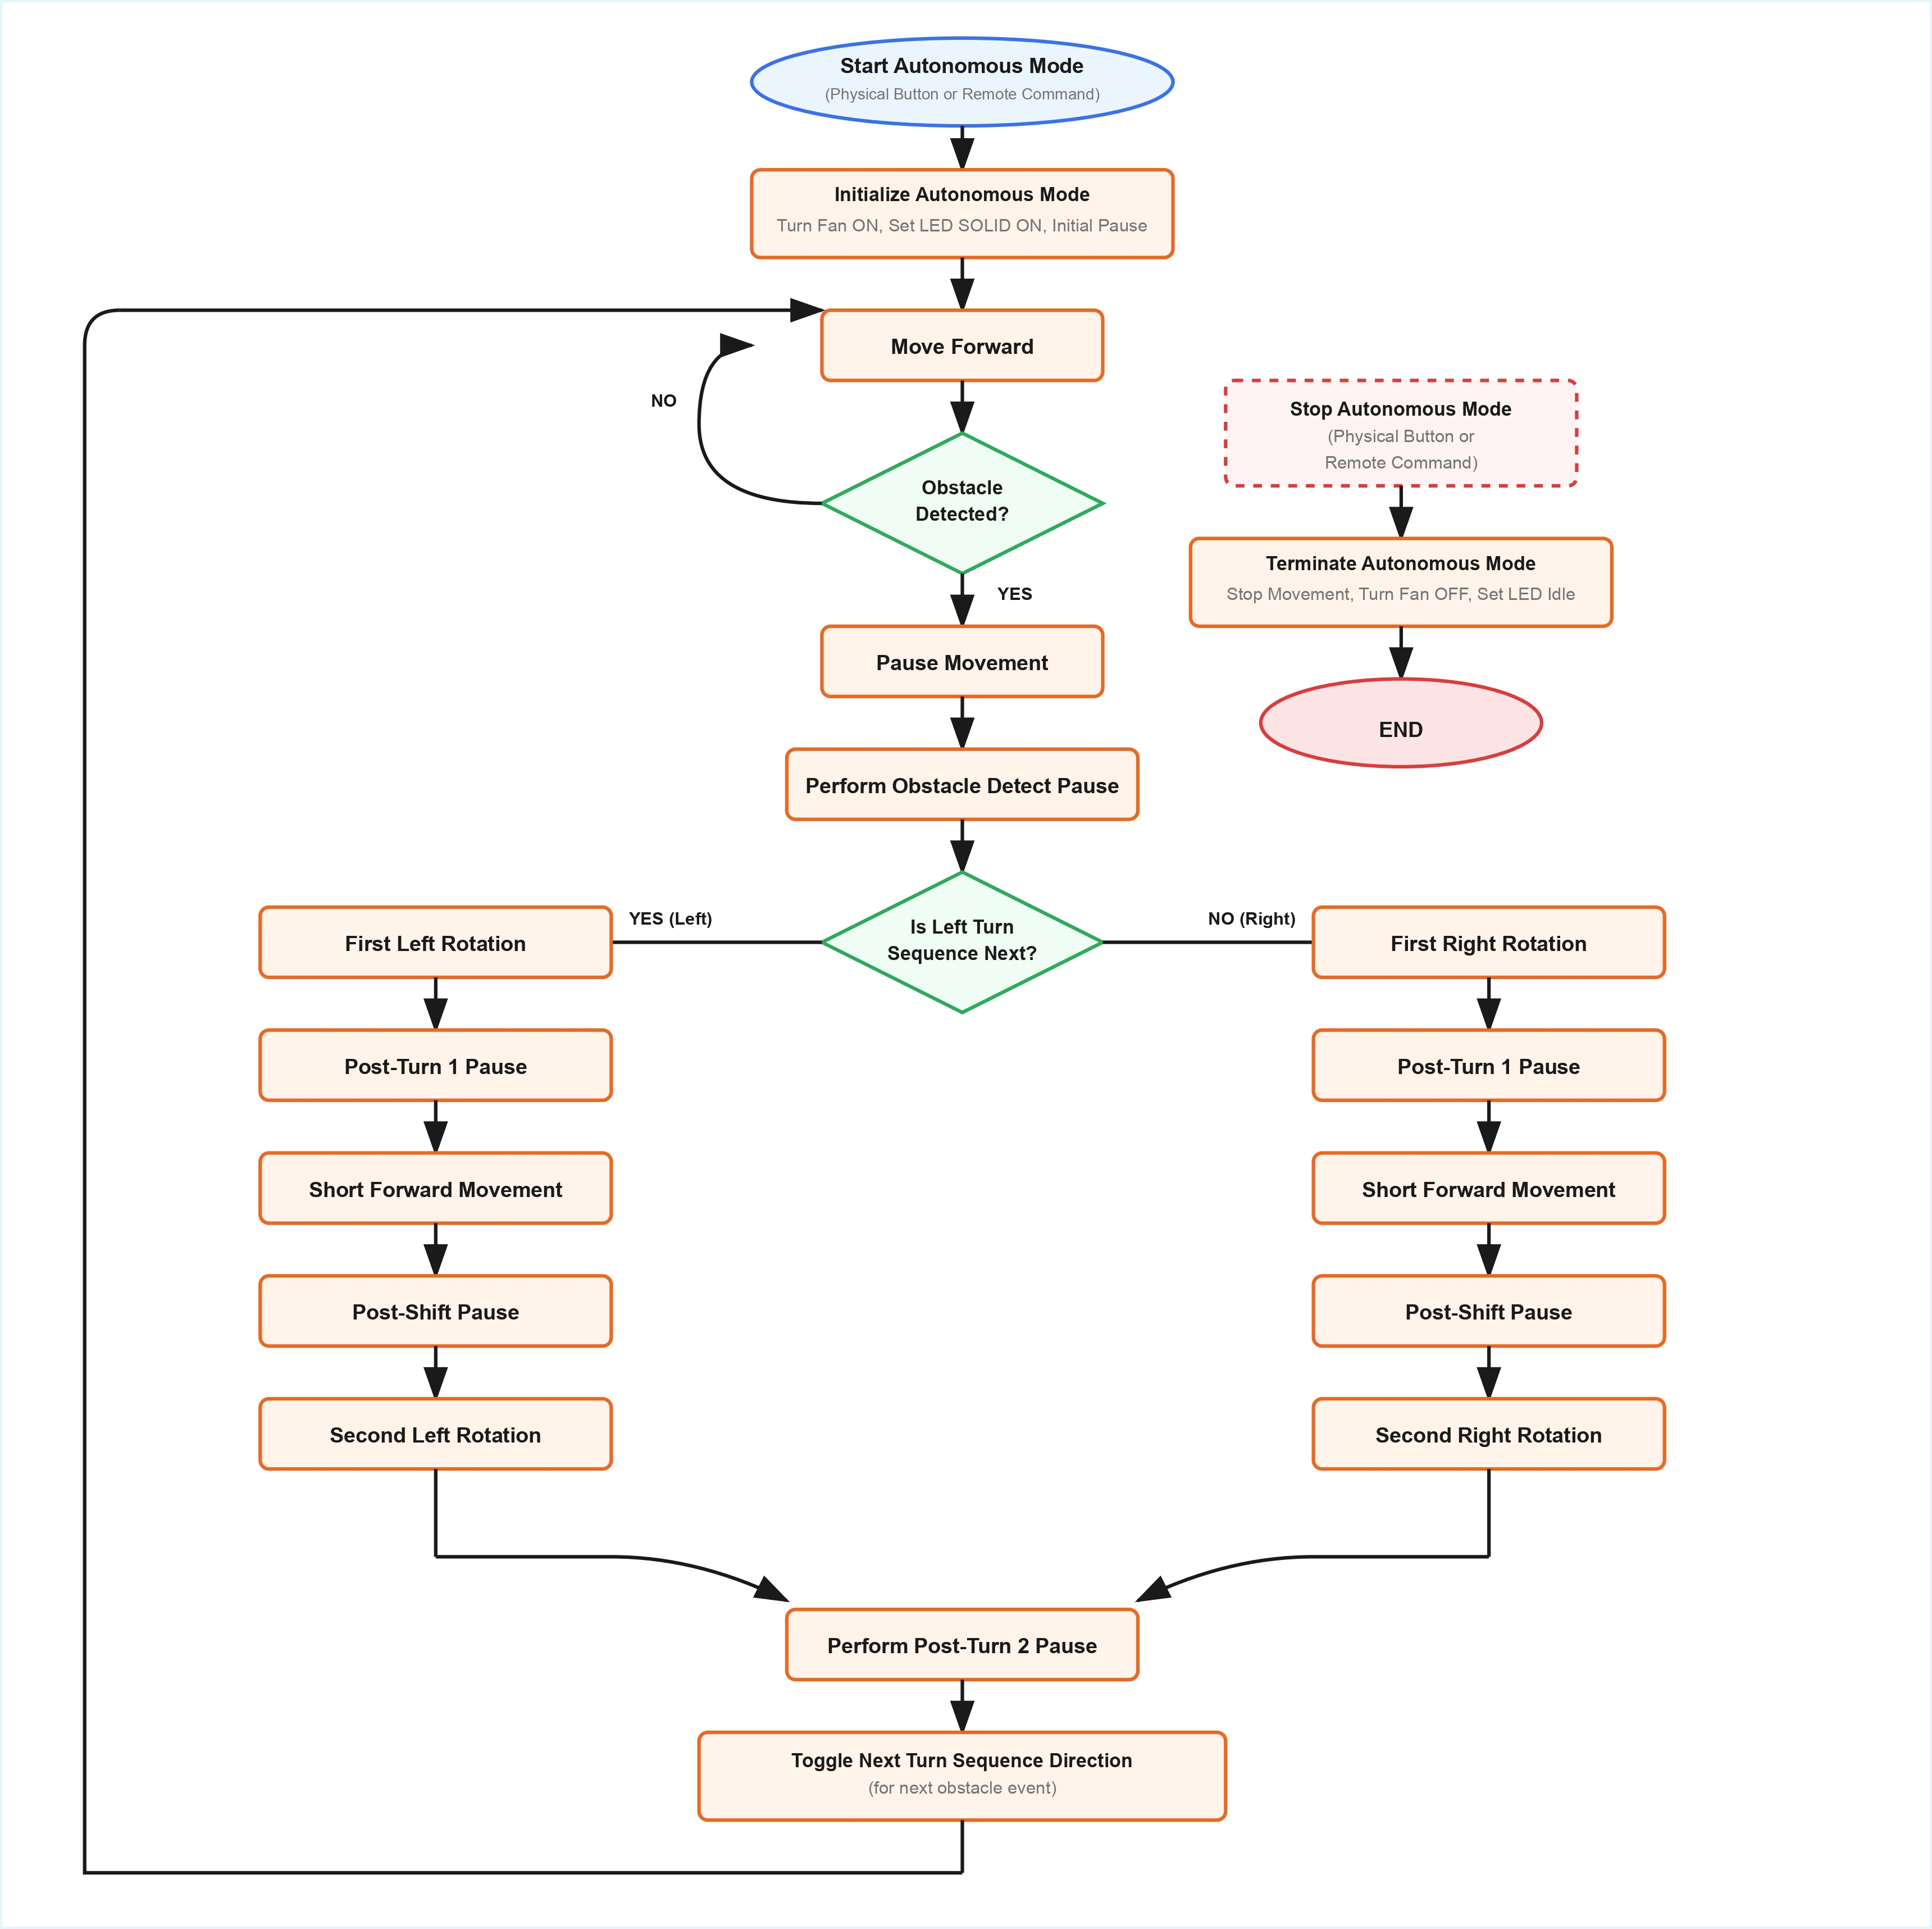
\includegraphics[width=0.85\textwidth]{images/screenshots/software_flowchart.jpg}
    \caption{Block diagram of the autonomous obstacle-avoidance state machine showing the robot's operational states and transitions.}
    \label{fig:flowchart_autonomous_logic_ctrl_new}
\end{figure}


\subsection{Evolution of the Control Strategy}
\label{subsec:control_strategy_evolution}
The initial navigation strategy was purely reactive and time-based, which lacked precision. The introduction of wheel encoders enabled a more sophisticated, closed-loop system. The development evolved from a pure feedback approach to a more robust hybrid model.

\subsubsection{Limitation of Pure \texorpdfstring{\hyperref[term:pid]{PID}}{PID} Control}
The first closed-loop attempts used a \textbf{Positional \hyperref[term:pid]{PID}} controller. This controller's error term was calculated from the difference in the total distance traveled by each wheel (\texttt{left\_pulses - right\_pulses}) to actively correct for drift. While a significant improvement, this purely reactive system was susceptible to a critical hardware limitation: aggressive \hyperref[term:pid]{PID} adjustments, especially during turns, would attempt to draw excessive current to compensate for motor differences. This led to voltage sags (\textbf{brownouts}) that would stall a motor, causing the control system to fail catastrophically. This discovery highlighted that a superior software algorithm can be defeated by the physical limitations of its hardware.

\subsubsection{Final Implemented Architecture: Hybrid Feed-Forward and \texorpdfstring{\hyperref[term:pid]{PID}}{PID} Control}
To create a more robust system, a \textbf{hybrid feed-forward and feedback} architecture was developed, as reflected in the accompanying source code (\texttt{main.py}).
\begin{itemize}
    \item \textbf{Feed-Forward (FF) Model}: A simple linear model (\texttt{ff\_pwm}) was created to proactively estimate the required \hyperref[term:pwm]{PWM} signal for a given target speed (in pulses per second). This forms the primary, anticipatory part of the controller, providing the ``muscle'' for a given movement based on the desired outcome.
    \item \textbf{\hyperref[term:pid]{PID} as a Correction Layer}: The positional \hyperref[term:pid]{PID} controller was retained but repurposed. Instead of calculating the entire motor command, it now calculates a small \textit{adjustment} to the target speed. This feedback layer acts as a fine-tuner, correcting for small, unmodeled errors (e.g., wheel slip, friction changes) without making the large, aggressive power demands that previously caused system instability.
    \item \textbf{Manual Control Enhancement}: The manual control logic was updated to a toggle system. Sending a movement command (e.g., ``FORWARD'') initiates the motion; sending the same command a second time applies the brake and stops the robot, providing more intuitive control.
    \item \textbf{Stall Detection and Recovery}: A safety-critical routine was integrated. During autonomous movement, the software checks if the encoder pulses have stopped. If the robot is physically stuck, it triggers a recovery state where it reverses and turns to free itself.
\end{itemize}
This journey from a simple reactive system to a hardware-aware hybrid controller demonstrates a comprehensive engineering process of design, testing, diagnosis, and refinement.

\subsubsection{PID Tuning Methodology}
\label{subsubsec:pid_tuning}
The \hyperref[term:pid]{PID} gains ($K_p$, $K_i$, $K_d$) were determined through an empirical trial-and-error process, a practical approach suitable for this prototype. The tuning followed a systematic procedure:
\begin{enumerate}
    \item \textbf{Start with P only}: Initially, only proportional gain was applied. The value was increased until oscillation occurred, then reduced.
    \item \textbf{Add D for damping}: Derivative gain was introduced to reduce overshoot and smooth the response.
    \item \textbf{Add minimal I}: A small integral term was added to eliminate steady-state drift, with careful limiting to prevent windup.
\end{enumerate}
The final tuned values for the positional correction \hyperref[term:pid]{PID} were conservative (low gains) to avoid the brownout conditions described earlier. This trade-off prioritized system stability over aggressive correction, accepting slightly less precise correction in exchange for reliable operation.

\subsection{\texorpdfstring{\hyperref[term:ble]{BLE}}{BLE} Remote Control}
\label{subsec:ble_remote_control_ctrl_new} % Relabelled from old subsec:ble_remote_control_ctrl
The Raspberry Pi Pico W's \hyperref[term:ble]{BLE} capability is utilized for manual remote control. A \hyperref[term:ble]{BLE} \hyperref[term:uart]{UART} service is implemented on the Pico W, allowing it to receive commands from a connected \hyperref[term:ble]{BLE} central device, typically a smartphone running a compatible application.
\subsubsection*{NRF Toolbox Application}
For this project, the NRF Toolbox application (or a similar \hyperref[term:ble]{BLE} \hyperref[term:uart]{UART} terminal app) can be used to interact with the robot. The application connects to the Pico W's \hyperref[term:ble]{BLE} service and allows the user to send text-based commands over the \hyperref[term:uart]{UART} profile.
\begin{itemize}
    \item \textbf{Connection}: The user scans for \hyperref[term:ble]{BLE} devices and connects to the robot, which advertises with a unique name (e.g., ``PicoRobot-3C33'').
    \item \textbf{Command Interface}: The \hyperref[term:uart]{UART} interface in the NRF Toolbox app provides a console or programmable buttons to send specific string commands to the robot. The MicroPython code on the Pico W (\texttt{main.py}) is programmed to recognize commands such as ``FORWARD'', ``BACKWARD'', ``LEFT'', ``RIGHT'', ``CLEAN'', ``FAN'', and ``HORN''. A key feature of manual control is that sending the same movement command twice acts as a toggle, stopping the robot.
    \item \textbf{Functionality}: This setup enables direct manual control of the robot's movements and functions, providing an alternative to the autonomous mode and facilitating testing or direct intervention.
\end{itemize}
Figure~\ref{fig:nrf_toolbox_ui_new} shows an example user interface. The integration of \hyperref[term:ble]{BLE} significantly enhances the robot's usability and interactivity.

\subsubsection*{Safety Feature - Manual Obstacle Block}
The system implements a safety feature for manual forward movement. If the user commands the robot forward but the ultrasonic sensor detects an obstacle, the software flags the robot as blocked. It stops the motors and activates a buzzing sound to alert the user, preventing a collision. The user must then command a different direction (e.g., backward or turn) to clear the flag.


\begin{figure}[htbp]
    \centering
    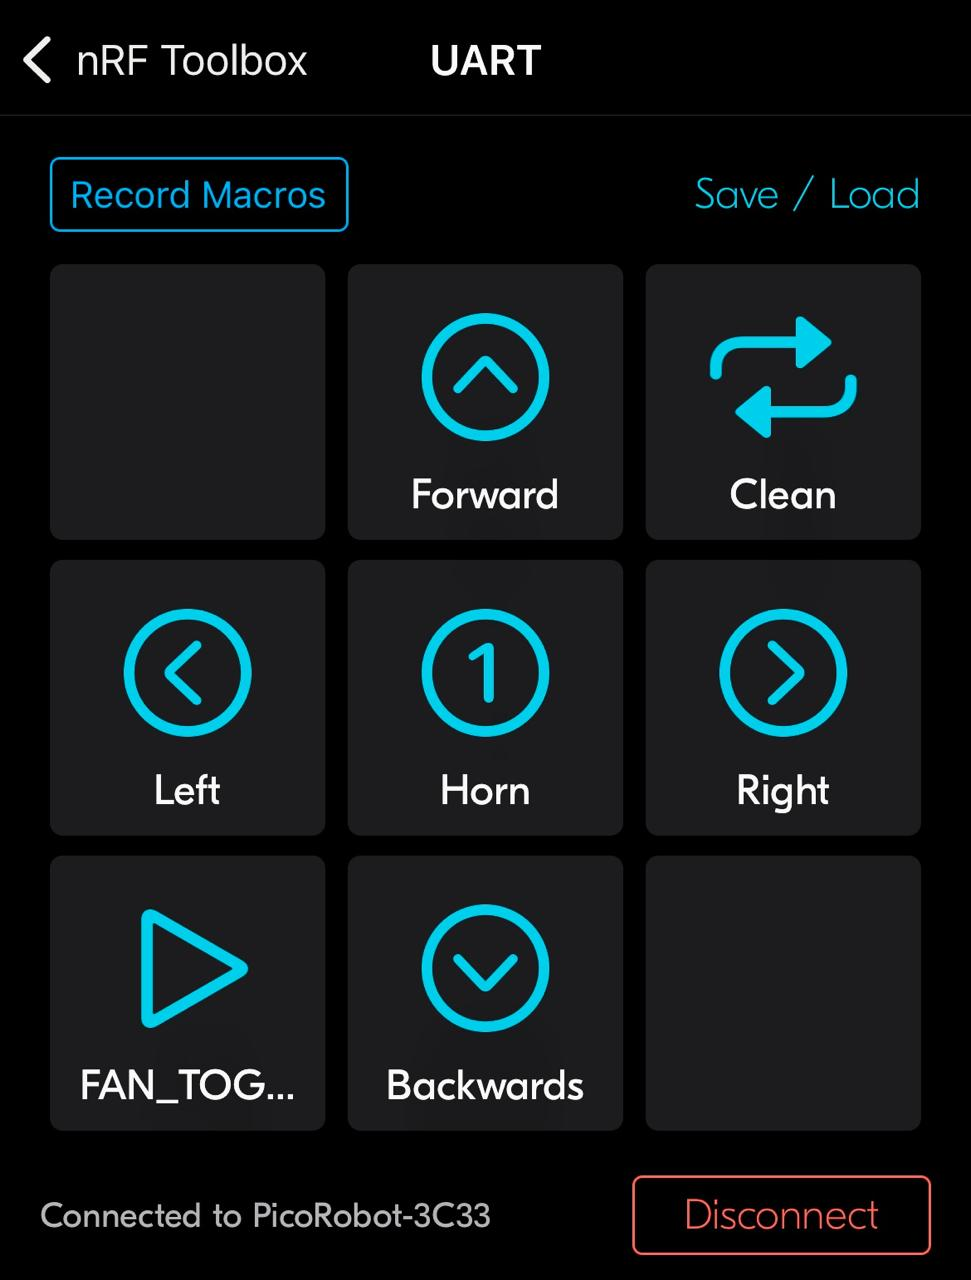
\includegraphics[width=0.401\textwidth, keepaspectratio]{images/screenshots/nrf_toolbox_ui.jpg}
    \caption{Example user interface of the NRF Toolbox application configured for controlling the Smart Cleaning Robot via BLE UART.}
    \label{fig:nrf_toolbox_ui_new} % Relabelled from fig:nrf_toolbox_ui
\end{figure}

\subsection{Software Deployment}
\label{subsec:software_deployment_new}
The MicroPython firmware was flashed onto the Raspberry Pi Pico W. The control script (\texttt{main.py}) was uploaded using the Thonny \hyperref[term:ide]{IDE}, as shown in Figure~\ref{fig:thonny_ide_screenshot_eval_new}. A \texttt{boot.py} script was configured to enable WebREPL for wireless debugging and parameter tuning during development.
\begin{figure}[htbp]
    \centering
    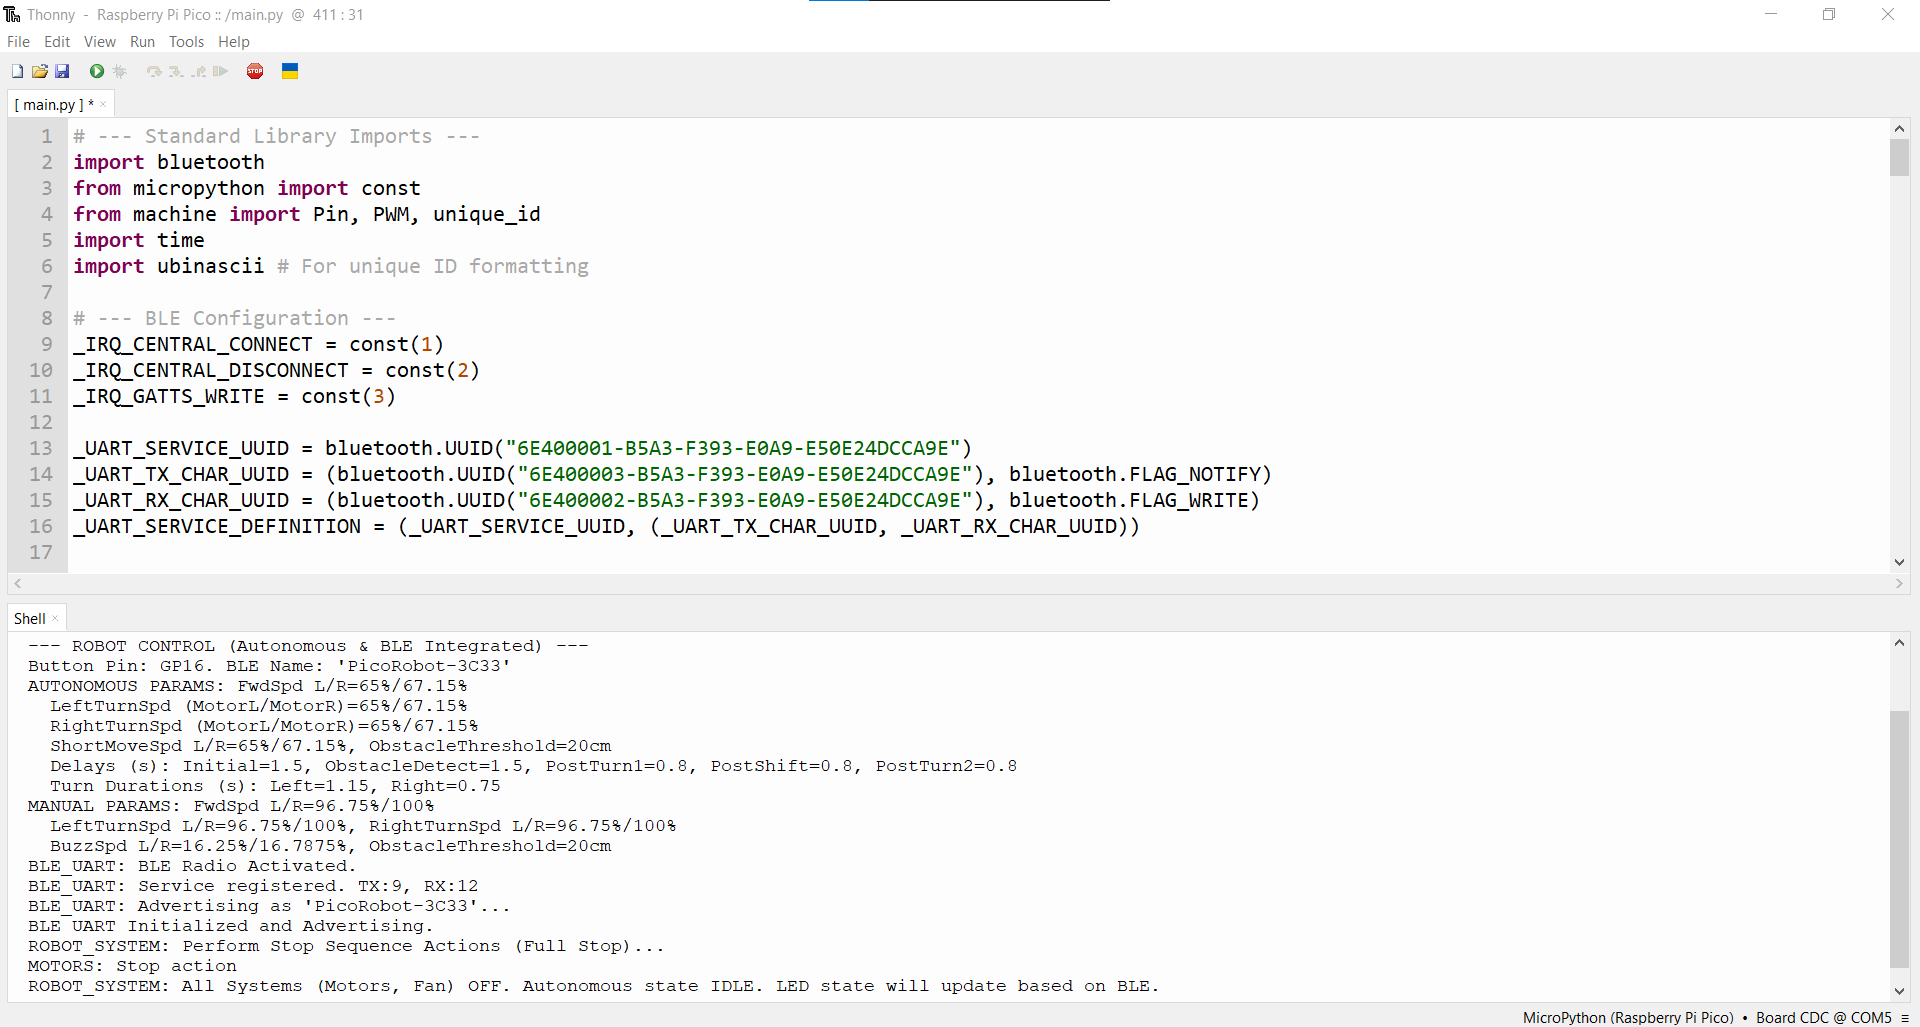
\includegraphics[width=0.85\textwidth, keepaspectratio]{images/screenshots/thonny_ide.png}
    \caption{Screenshot of Thonny IDE showing the MicroPython control script deployed to the Raspberry Pi Pico W.}
    \label{fig:thonny_ide_screenshot_eval_new} % Relabelled from fig:thonny_ide_screenshot_eval
\end{figure}


\section{Performance Evaluation and Results}
\label{sec:performance_evaluation_eval_new}

The evaluation focused on functional verification of core features and qualitative observation of the robot's behavior in a typical indoor test environment.
\subsection{Functional Verification and Observations}
\label{subsec:functional_verification_observations_new}

\begin{itemize}
    \item \textbf{Manual \hyperref[term:ble]{BLE} Remote Control}: Functioned perfectly. The robot exhibited prompt and accurate responses to commands sent via the NRF Toolbox application, with good connection stability over several meters. The \hyperref[term:pid]{PID}-assisted forward command was noticeably straighter than unassisted control.
    \item \textbf{Autonomous Navigation}: The integration of wheel encoders and a \hyperref[term:pid]{PID} control system resulted in a significant improvement in navigational accuracy over the previous open-loop system. Straight-line movement was noticeably more stable, with the positional \hyperref[term:pid]{PID} controller effectively mitigating much of the drift caused by motor and surface inconsistencies. While not perfectly precise in all scenarios, the robot could now execute its back-and-forth cleaning pattern more reliably. The dual-objective \hyperref[term:pid]{PID} controller produced more consistent turn angles. Furthermore, the newly implemented stall detection and recovery feature was tested and found to be effective in simulated ``stuck'' conditions.
    \item \textbf{Vacuum System Performance}:
        \begin{itemize}
            \item \textit{Debris Collection:} The vacuum system, using the PS3 fan, collected light debris like small paper pieces and dust from hard floor surfaces.
            \item \textit{Limitations:} Performance was constrained by two main factors: the absence of a check valve, leading to occasional spillage of collected debris at the end of an operation, and the unavailability of brushes, which limited the robot's ability to dislodge embedded dirt.
        \end{itemize}
    \item \textbf{Power System}: The 12V \hyperref[term:liion]{Li-ion} battery pack~\cite{BatteryPack12V4000mAhDatasheet} and LM2596S buck converter provided stable power, achieving an operational runtime exceeding 60 minutes on a full charge during continuous autonomous operation. The overall system current and power are approximately \totalCurrent{} and \totalPower{} respectively, at a nominal \totalVoltage{}. This estimate is based on the main power-consuming components: the PS3 fan (rated $\sim$1.3A at 12V), and the two DC motors, which can draw over 0.8A combined under operational load. The remaining electronics contribute a smaller fraction to the total consumption. Peak current during motor startup or simultaneous operation of all high-draw components could be higher.
    \item \textbf{User Interface (Button/\hyperref[term:led]{LED})}: The physical start/stop button and status \hyperref[term:led]{LED} functioned as designed, providing correct user interaction and feedback.
\end{itemize}

Table~\ref{tab:test_results} summarizes the key performance metrics observed during testing.

\begin{table}[htbp]
\centering
\caption{Performance Test Results Summary.}
\label{tab:test_results}
\begin{tabular}{|l|c|l|}
\hline
\textbf{Metric} & \textbf{Result} & \textbf{Notes} \\ \hline
BLE Connection Range & $>$5 m & Stable indoor connection \\ \hline
Straight-Line Stability & Good & PID reduces drift significantly \\ \hline
Turn Angle Consistency & Improved & More reliable than open-loop \\ \hline
Stall Detection & Functional & Recovery sequence works \\ \hline
Battery Runtime & $>$60 min & Continuous operation \\ \hline
Debris Collection & Light debris & Paper, dust on hard floors \\ \hline
System Power & $\sim$26W & At \totalVoltage{} nominal \\ \hline
\end{tabular}
\end{table}
\subsection{Summary}
\label{subsec:discussion_performance_evaluation_new}

The performance evaluation indicates that the upgrade to a closed-loop, \hyperref[term:pid]{PID}-based control system was a success. While not achieving perfect motion, it dramatically improved the precision and reliability of the robot's movement compared to the initial prototype. The implemented control system enabled the robot's autonomous behavior to be more systematic and, crucially, allowed for the integration of vital safety features like stall detection and recovery. The custom \hyperref[term:pcb]{PCB} and overall physical construction represent a solid prototyping effort.

The evaluation also confirms that achieving flawless path execution with the current DC motor and chassis setup remains a challenge. The vacuum system, while functional for light debris, also has clear limitations impacting its practical cleaning effectiveness. These findings are valuable insights that directly inform the recommendations for future work.
